%%=============================================================================
%% Methodologie
%%=============================================================================

\chapter{Methodologie}
\label{ch:methodologie}

%% TODO: Hoe ben je te werk gegaan? Verdeel je onderzoek in grote fasen, en
%% licht in elke fase toe welke stappen je gevolgd hebt. Verantwoord waarom je
%% op deze manier te werk gegaan bent. Je moet kunnen aantonen dat je de best
%% mogelijke manier toegepast hebt om een antwoord te vinden op de
%% onderzoeksvraag.

Aangezien er verschillende soorten types zijn van blockchains wordt ook elk type toegepast op de usecase. Er worden dus bestanden toegevoegd aan de blockchain door transacties uit te voeren. Dit systeem zal vervolgens uitwerken en de voordelen en nadelen aankaarten van elk type blockchain. De werking van hoe we juist een bestand gaan toevoegen aan de chain zal in het algemeen hetzelfde blijven en dit wordt dan ook bekijken in hoofdstuk \ref{ch:add-to-blockchain}. Vooral de werking tussen de verschillende nodes zal veranderen aangezien er telkens een ander overeenkomst algoritme zal gebruikt worden. Een ander verschil is ook dat er enerzijds documenten zoals contracten en dergelijke op een publiek netwerk zullen geplaatst worden en anderzijds op een privé netwerk. Hierdoor zal er tot 1 enkele of meerdere optimale oplossingen gekomen worden afhankelijk van de opstelling en het standpunt.

Verder zullen er ook enkele tegenhangende technologieën besproken worden zoals hashgraph in hoofdstuk \ref{ch:alternative-technology}. Deze zal niet intensief onderzocht worden maar zal toch ook enkele verbeterde punten aantonen of enkele minpunten aantonen. 

Tenslotte zal uit dit onderzoek onze conclusie getrokken worden en wordt bekeken welk type blockchain het meeste geschikt zou zijn om gevoelige data veilig te houden en zo optimaal mogelijk en kost effectief te laten werken. Vervolgens zal  ook de studie van de alternatieve technologiën bekeken worden en wordt er een conclusie getrokken welke technologie juist het meest geschikt is. 


%%=============================================================================
%% Literatuurstudie
%%=============================================================================

\chapter{Blockchain}
\label{ch:blockchain}

%% TODO: deze sectie (die je kan opsplitsen in verschillende secties) bevat je
%% literatuurstudie. Vergeet niet telkens je bronnen te vermelden!`

\section{Wat is blockchain?}

Blockchain is een technologie die het best kan vergeleken worden met een database. Het wordt dan ook vooral gebruikt om gevoelige data veilig op te slaan. Blockchain dook voor het eerst op in het Bitcoin whitepaper door \textcite{Nakamoto2008}, dit blijkt een alias te zijn voor een persoon of een groep en de echte ontwikkelaar is niet gekend bij naam. Uit dit document kan afgeleid worden dat het gaat om een enkel persoon maar dit is niet met zekerheid geweten. 

Blockchain is een peer-to-peer technologie of ook ``ledgers'' genoemd. Dit wil zeggen dat alle data niet in één plaats is opgeslagen maar op verschillende servers of ook nodes genoemd. Zo heeft elke node een versie van de blockchain. Dit is meteen ook één van de reden waarom blockchain zo veilig is en ook niet eenvoudig is om te hacken, bovendien is de blockchain volledig geëncodeerd door middel van een hash, deze verwijst naar het vorige blok en het volgende blok. Een voorbeeld van de hash is te zien in Figuur \ref{fig:blockchain-hash-example}. Hoe veilig deze technologie juist is wordt uitgelegd in een volgend hoofdstuk.

Blockchain is meteen ook de technologie achter het bekende Bitcoin. Het idee was om digitaal geld te kunnen transporteren van één partij naar een andere zonder de tussenkomst van een financiële instelling of dergelijke. Blockchain heeft dan ook het grote voordeel te werken met een peer-to-peer systeem wat waarschijnlijk raar klinkt voor een geld transport systeem aangezien banken werkten met een centraal systeem om veiligheid te garanderen. Dit heeft uiteraard ook vele nadelen zoals het integreren met andere platformen. Toch blijkt blockchain een veilige manier te zijn en dit door de manier van hoe blockchain werkt.

Blockchain is het makkelijkst voor te stellen als een excel-blad. Elke rij in het blad is een transactie, en de transactie heeft telkens een relatie met de vorige transactie. Dit is te zien op figuur \ref{fig:blockchain-transaction-example}. Zo kan er dus bijvoorbeeld geen 10.000 euro getoverd worden op een bitcoin rekening aangezien deze moet gestort worden met een transactie en dus wel degelijk ergens vandaan moet komen.

\begin{figure}
	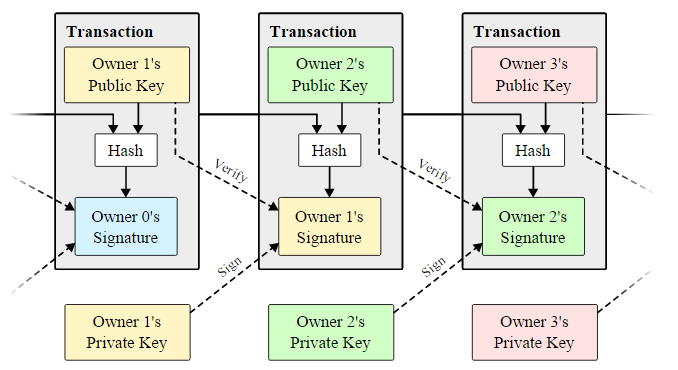
\includegraphics[width=\linewidth]{blockchaintransactions.png}
	\caption{Voorbeeld van transacties \textcite{Nakamoto2008}.}
	\label{fig:blockchain-transaction-example}
\end{figure}
\begin{figure}
	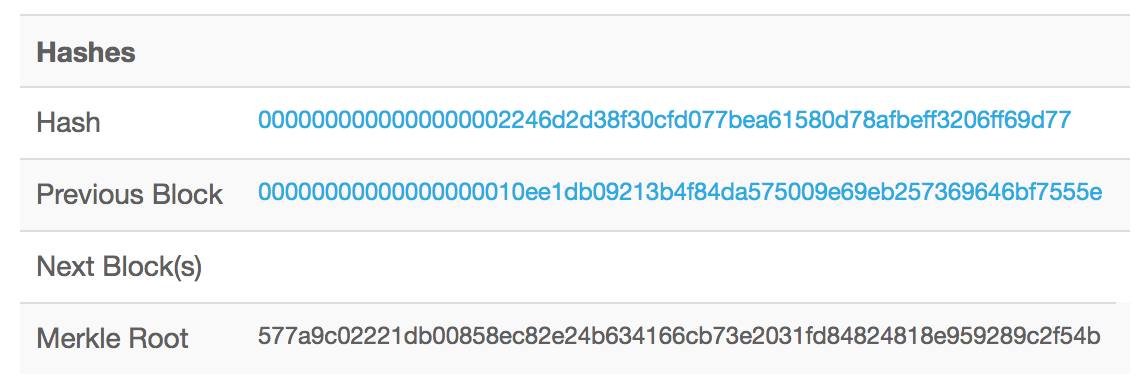
\includegraphics[width=\linewidth]{blockchain-hashes.png}
	\caption{Voorbeeld van hashes \textcite{blockchain.info}.}
	\label{fig:blockchain-hash-example}
\end{figure}

\subsection{Hoe wordt een blockchain geïnitialiseerd?}
Natuurlijk moet er wel een manier zijn om bijvoorbeeld nieuw geld in de blockchain toe te voegen, dit moet dan uiteraard wel ergens vandaan komen dus er moet natuurlijk wel een manier zijn om instanties aan te kunnen maken. 

De eerste transactie in een blok wordt gezien als een speciale transactie die meteen ook een nieuwe munt zal aanmaken waar hij eigenaar van is. Dus voor elke eerste transactie van een blok wordt een nieuwe munt aangemaakt waarvan de node dus eigenaar is. Dit zorgt meteen ook voor een goede reden om het netwerk van nodes te steunen en zorgt ook meteen voor een manier om nieuwe munten in omloop te brengen aangezien er geen centrale authoriteit is die de blockchain beheert. 

Er wordt dus constant geld toegevoegd aan de bitcoin blockchain als het gevolg van het verbruiken van middelen. In het geval van Bitcoin is dit bijvoorbeeld elektriciteit en CPU-kracht en dit zal voor de meeste blockchains ook het geval zijn. Dus met andere woorden wordt het openstellen van CPU-kracht en het gebruik hiervan beloond door het verkrijgen van bitcoins bij het aanmaken van een nieuw blok. Dit heeft ook als voordeel dat het proberen hacken van de blockchain niet meer zo gunstig zou zijn en het dus beter is om een ``eerlijke'' node te blijven. Natuurlijk is het niet nodig om steeds een nieuwe munt aan te maken als motivatie want dit zou zorgen voor inflaties. Wanneer er bijvoorbeeld een genoeg aantal munten in omloop zijn kan het gehele systeem van verbruikte middelen ook vergoed worden door transactiekosten zodat er helemaal geen inflatie optreedt.

\section{Kan iedereen zich aansluiten bij de nodes?}
Iedereen kan lid worden van een blockchain netwerk en CPU-kracht beschikbaar stellen wanneer de blockchain publiek is zoals dit bij Bitcoin het geval is, dit wordt ook ``gold miners'' genoemd in de Bitcoin blockchain. Een eigen computer ter beschikking stellen als node in het netwerk is mogelijk waardoor de gebruiker vergoed wordt met bitcoins. Deze zouden dan ook de kosten moeten dekken van de elektriciteit en de verbruikte CPU-kracht. Wie dus CPU-kracht over heeft kan deze ter beschikking stellen en hier aan verdienen. Op deze manier probeert  bitcoin bijvoorbeeld ook om alle nodes ``eerlijk'' te houden aangezien dit veel interessanter zou zijn. Het opstellen van een gold miner wordt later uitgelegd. 

Tegenwoordig kan dit niet meer door een eigen computer ter beschikking te stellen voor Bitcoin aangezien de verloning voor elektriciteit en CPU-kracht te laag zou zijn om dit competitief te houden. Daarom is er tegenwoordig hardware te koop om Bitcoins te minen (het verdienen van bitcoins) die hiervoor speciaal gemaakt zijn. Deze zijn meteen ook veel zuiniger \textcite{Bitcoinmining.com}.

\section{Soorten in blockchain}

\begin{figure}
	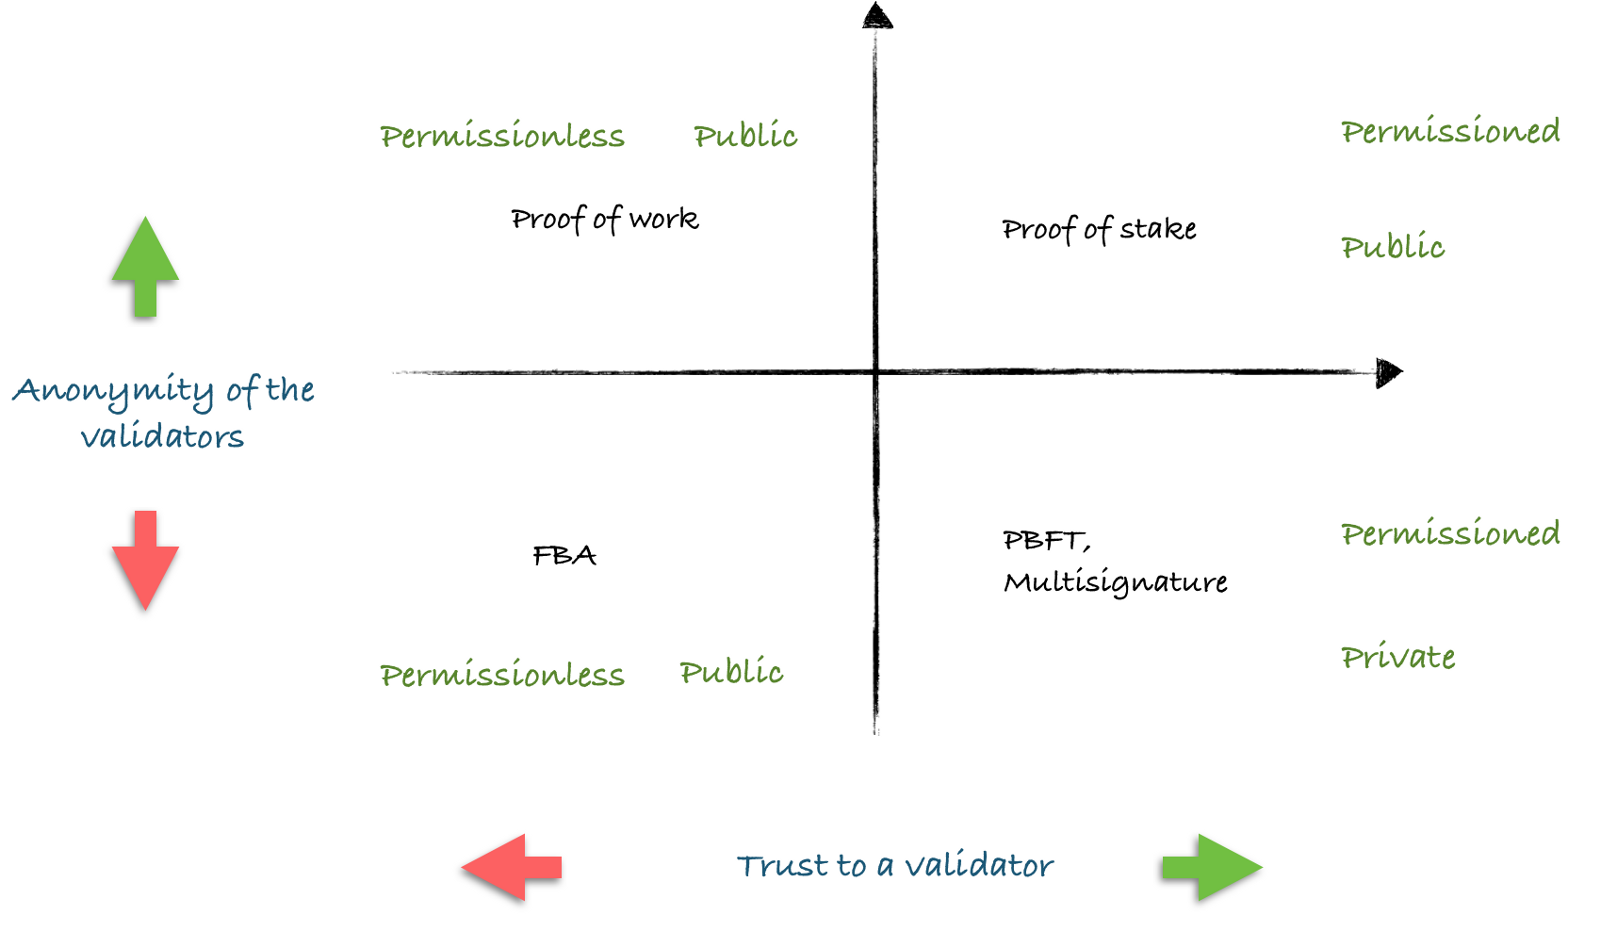
\includegraphics[width=\linewidth]{blockchain-types.png}
	\caption{Grafische voorstelling van verschillende blockchain opstellingen \textcite{Kravchenko2016}.}
	\label{fig:blockchain-types}
\end{figure}

Natuurlijk zijn er verschillende soorten blockchain. Doorheen de literatuurstudie wordt telkens Bitcoin als voorbeeld gebruikt, Bitcoin is uiteraard een publiek netwerk waar geen rechten op toegekend waren \textcite{Nakamoto2008}. Natuurlijk is dit niet de enige soort en zijn er nog andere varianten die telkens toch wat verschillen hebben. Hoofdzakelijk zijn er 2 veranderlijken, de anonimiteit en de hoeveelheid vertrouwen die de gebruiker heeft. \textcite{Kravchenko2016} maakte hierover een uitgebreid artikel en gebruikte het volgende schema dat te zien is op Figuur \ref{fig:blockchain-types}. Hier worden nodes weergegeven als validators.

Wie zien meteen dat Blockchain bovenaan links in de groep hoort. Niemand is gekend op het netwerk, er zijn geen rechten van toepassing en iedereen heeft toegang. De enige manier van validatie die hier van toepassing is, is proof-of-work. Men moet dus nooit op voorhand hebben deelgenomen of doorgelicht geweest zijn om deel te kunnen nemen. Het vertrouwen dat aan een ``miner'' (een node wordt bij bitcoin ook een miner genoemd) wordt gegeven is laag en er is ook geen straf voor het aanvallen van het systeem buiten het feit dat de mining apparatuur (hardware die geschikt is om gebruikt te worden als node) niet verder kan gebruikt worden als de aanval succesvol was. Dit type is dus vooral geschikt voor volledig anonieme systemen die volledig buiten een overheidinstanties werken. 

Bovenaan rechts is een publieke blockchain maar deze keer wel met rechten. Dit omdat er munten moeten gekocht worden om te kunnen minen. Een munt is dan ook iets wat van het systeem zelf is en niet werkt zoals Bitcoin waar een munt wordt gegeven aan de eigenaar van mining machines. Deze soort beveiliging wordt ook ``proof of stake'' genoemd. Dit soort systemen geven hierdoor ook meer vertrouwen aan de gebruiker aangezien bij een aanval op het syteem de ``borg'' verloren gaat bij het proberen uitvoeren van een aanval of dubbele uitgave. Dit soort systemen is ideaal voor de uitvoering van contracten, gemeenschapsbestuur, privé geld systemen, enz. 

Onderaan links bevindt zich een andere publike blockchain zonder regels. Onder bepaalde sociale overeenkomsten kan iedereen toegang krijgen tot het syteem en dus een node worden in het systeem. Een goed voorbeeld hiervan is bijvoorbeeld een land waar elke bewoner het recht heeft om een node te worden van het netwerk. Het vertrouwen dat wordt gegeven aan een node is vrij laag, zelfs met de identiteit die gekend is. Dit is meteen ook een groot verschil met de bitcoin variant waar iedereen niet gekend is. Hoe komen systemen dan overeen bij validatie van data? In praktijk toont dat een FBA (Federated Byzantine Agreement) overeenkomst het beste is in de meeste gevallen. Proof of stake kan hier bijvoorbeeld niet gebruikt worden aangezien elke node evenveel inspraak heeft. Dit zou bijvoorbeeld goed werken voor nationale blockchains en dergelijke. 

Als laatste blijft het kwadrant over dat onderaan rechts ligt. Dit kwadrant bevat de blockchain die volledig afgeschermd is, dus volledige privé en met regels. Om te kunnen deelnemen moet men dus een soort licentie hebben of deel zijn van een groep. Deze soort van blockchain is vooral bruikbaar in bedrijven, banken en andere zaken. Overeenkomst tussen de systemen kan snel gebeuren aangezien er veel vertrouwen wordt gegeven aan de nodes, een aanval op het systeem zorgt dan ook meteen voor het verliezen van de licentie en dus toegang of het verwijderd worden uit de groep. Als validatie overeenkomst tussen de nodes wordt PBFT of multisignature gebruikt. Een groot voordeel zoals eerder vermeld is het snel afhandelen van overeenkomsten. 

\section{Transacties en validatie.}
Hoe wordt er voorkomen dat er illegale transacties worden uitgevoerd? Het hele systeem werkt op basis van peer-to-peer, elke node heeft dus zijn eigen versie. Telkens er een verandering wordt uitgevoerd dan wordt de blockchain blok gebroadcast over het hele netwerk. Vervolgens gaat elke node die de transactie ontving deze gaan plaatsen in een blok. Elke node zal vervolgens een moeilijke proof-of-work genereren of gebruik maken van een ander algoritme. Wanneer een node de transactie heeft goedgekeurd zal hij deze blok versturen naar alle andere nodes in het netwerk. Er zijn verschillende  algoritmen die gebruikt kunnen worden om een consensus te bereiken. Vervolgens zullen de nodes het blok enkel en alleen aanvaarden als alle transacties in het blok kloppen en nog niet vervallen zijn. Om aan te tonen dat een node het blok heeft aanvaard zal deze node de hash van dit blok gebruiken in het volgende blok als vorige hash. 

\begin{figure}
	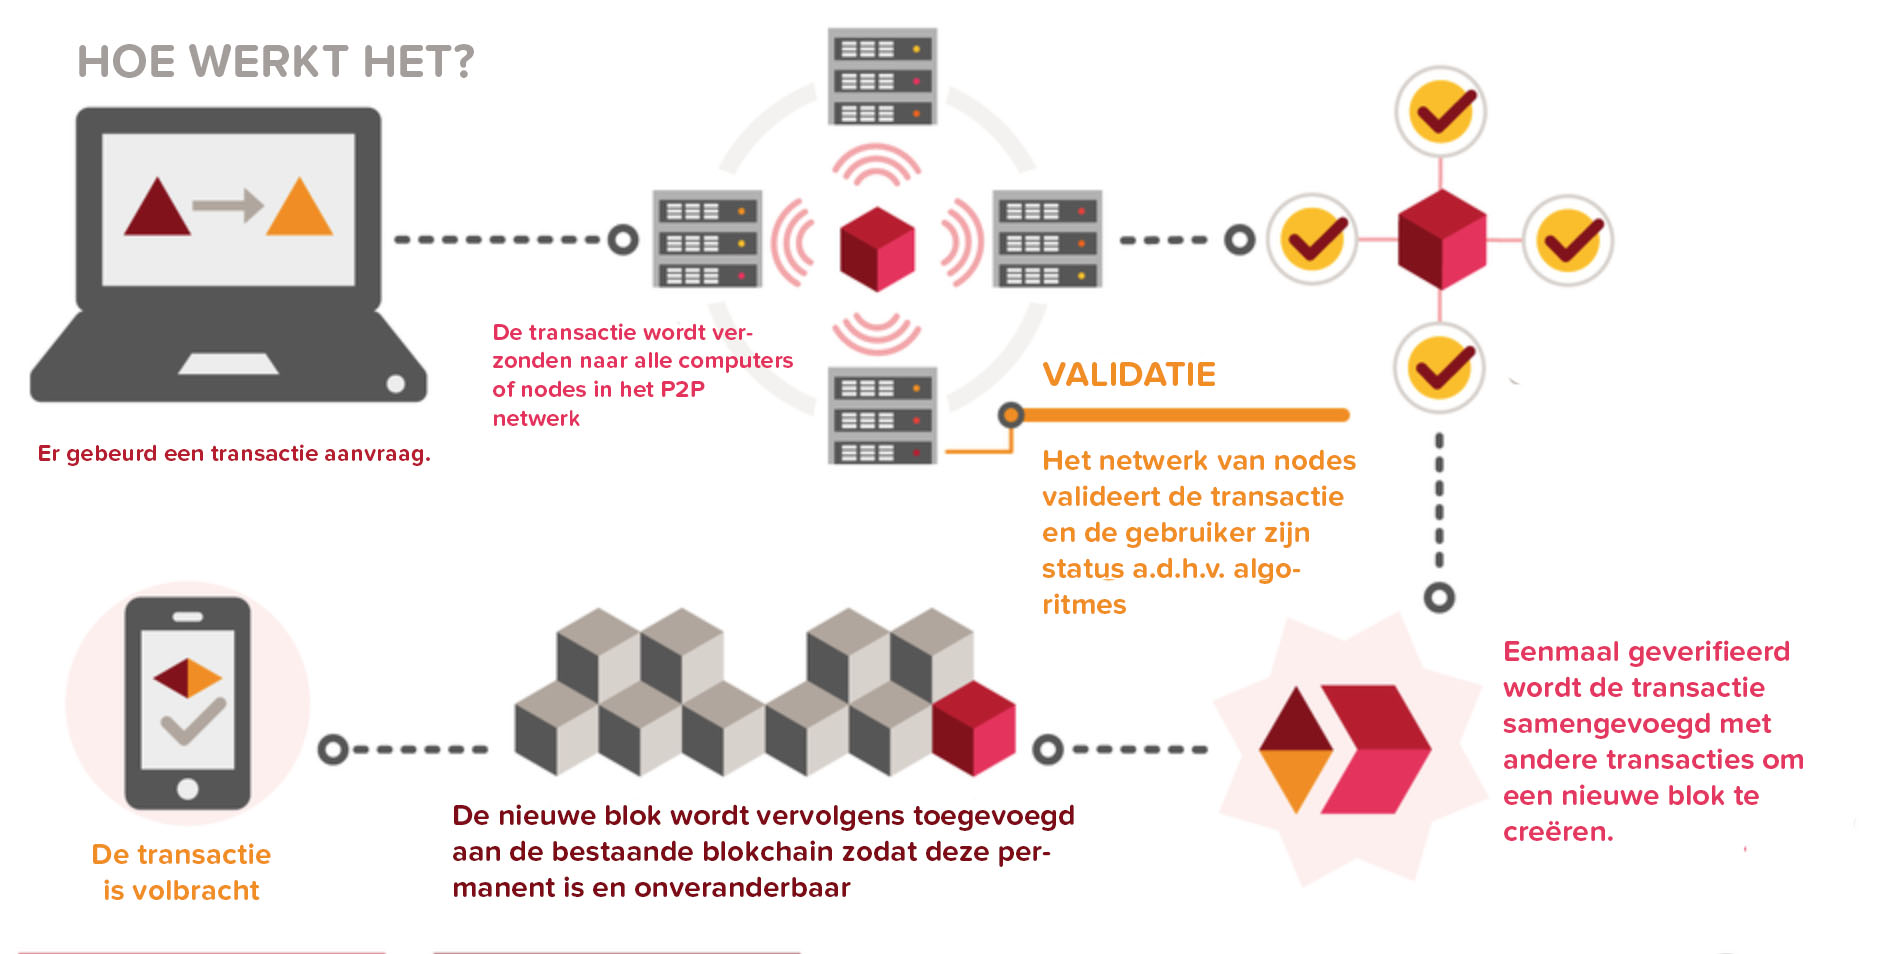
\includegraphics[width=\linewidth]{blockchain-howto.jpg}
	\caption{Grafische voorstelling van de werking van blockchain \textcite{pwc.com}.}
	\label{fig:blockchain-howto}
\end{figure}

In het algemeen zullen de nodes altijd de langste ``ketting'' aanvaarden als de correcte en zullen ze verder werken aan deze ketting. Wanneer twee nodes een verschillend blok gaan broadcasten dan kan het zijn dat één node de ene versie eerst zal krijgen en een andere de alternatieve versie eerst zal ontvangen. Daarom zal altijd het eerste dat ontvangen werd gebruikt worden. De alternatieve versie wordt dan bijgehouden. Deze koppeling wordt onderbroken vanaf er een nieuwe proof-of-work wordt gevonden. Hierdoor zal één van de twee versies langer worden en de langste versie zal dan gebruikt worden om op verder te bouwen. De nodes die ondertussen op de andere tak aan het werken waren zullen dan ook overschakelen op deze. Dit wil natuurlijk niet zeggen dat een transactie broadcast alle nodes moeten bereiken, het blijft steeds het internet en een transactie kan verloren geraken. Dit is geen probleem zolang er maar genoeg nodes de transactie ontvangen en deze verifiëren. De nodes die die transactie niet ontvingen zullen dit merken wanneer ze de volgende blok ontvangen en zien dat ze er één hebben gemist en zal deze dan aanvragen aan de andere nodes in het netwerk. De volledige werking is visueel weergegeven op Figuur \ref{fig:blockchain-howto}

Uiteraard kan het ook soms de bedoeling zijn dat bepaalde data niet gezien mag worden op het netwerk. Hiervoor kan gebruik gemaakt worden van enkele cryptografische functies die los gelaten worden op de gegevens en deze versleutelen. Een voorbeeld hiervan en momenteel ook meeste gebruikte algoritme  is Sha-256. 

\subsection{Wat is SHA-256}
SHA-2 is een verzameling van cryptografische hash functies die gemaakt werden door de National Security Agency (NSA). Cryptografische hash functies zijn wiskundige bewerkingen die kunnen uitgevoerd worden op digitale data. Door vervolgens de berekende ``hash'' te vergelijken met de verwachte hash kan men de data integriteit bepalen \textcite{Fisher2017}. Om dit principe te verduidelijken nemen we het volgende voorbeeld. Men heeft een bestand gedownload, laat ons zeggen dat dit een ``word'' bestand is. Men maakt vervolgens een kopie van dit bestand en passen in het word document enkele dingen aan.Vervolgens wordt het document opgeslagen en wordt de hash berekend van beide documenten. Nu heeft men dus het originele bestand en het aangepaste bestand. Als men nu de hash zouden vergelijken van beide documenten dan zal men zien dat deze verschillen. Mocht men nu van de originele versie nog een kopie maken en hiervan de hash berekenen dan zal deze dezelfde zijn van het originele bestand. Op deze manier kan men dus bekijken of een bestand gewijzigd is of niet. In Figuur \ref{fig:hash-example} wordt dit grafisch weergegeven.

\begin{figure}
	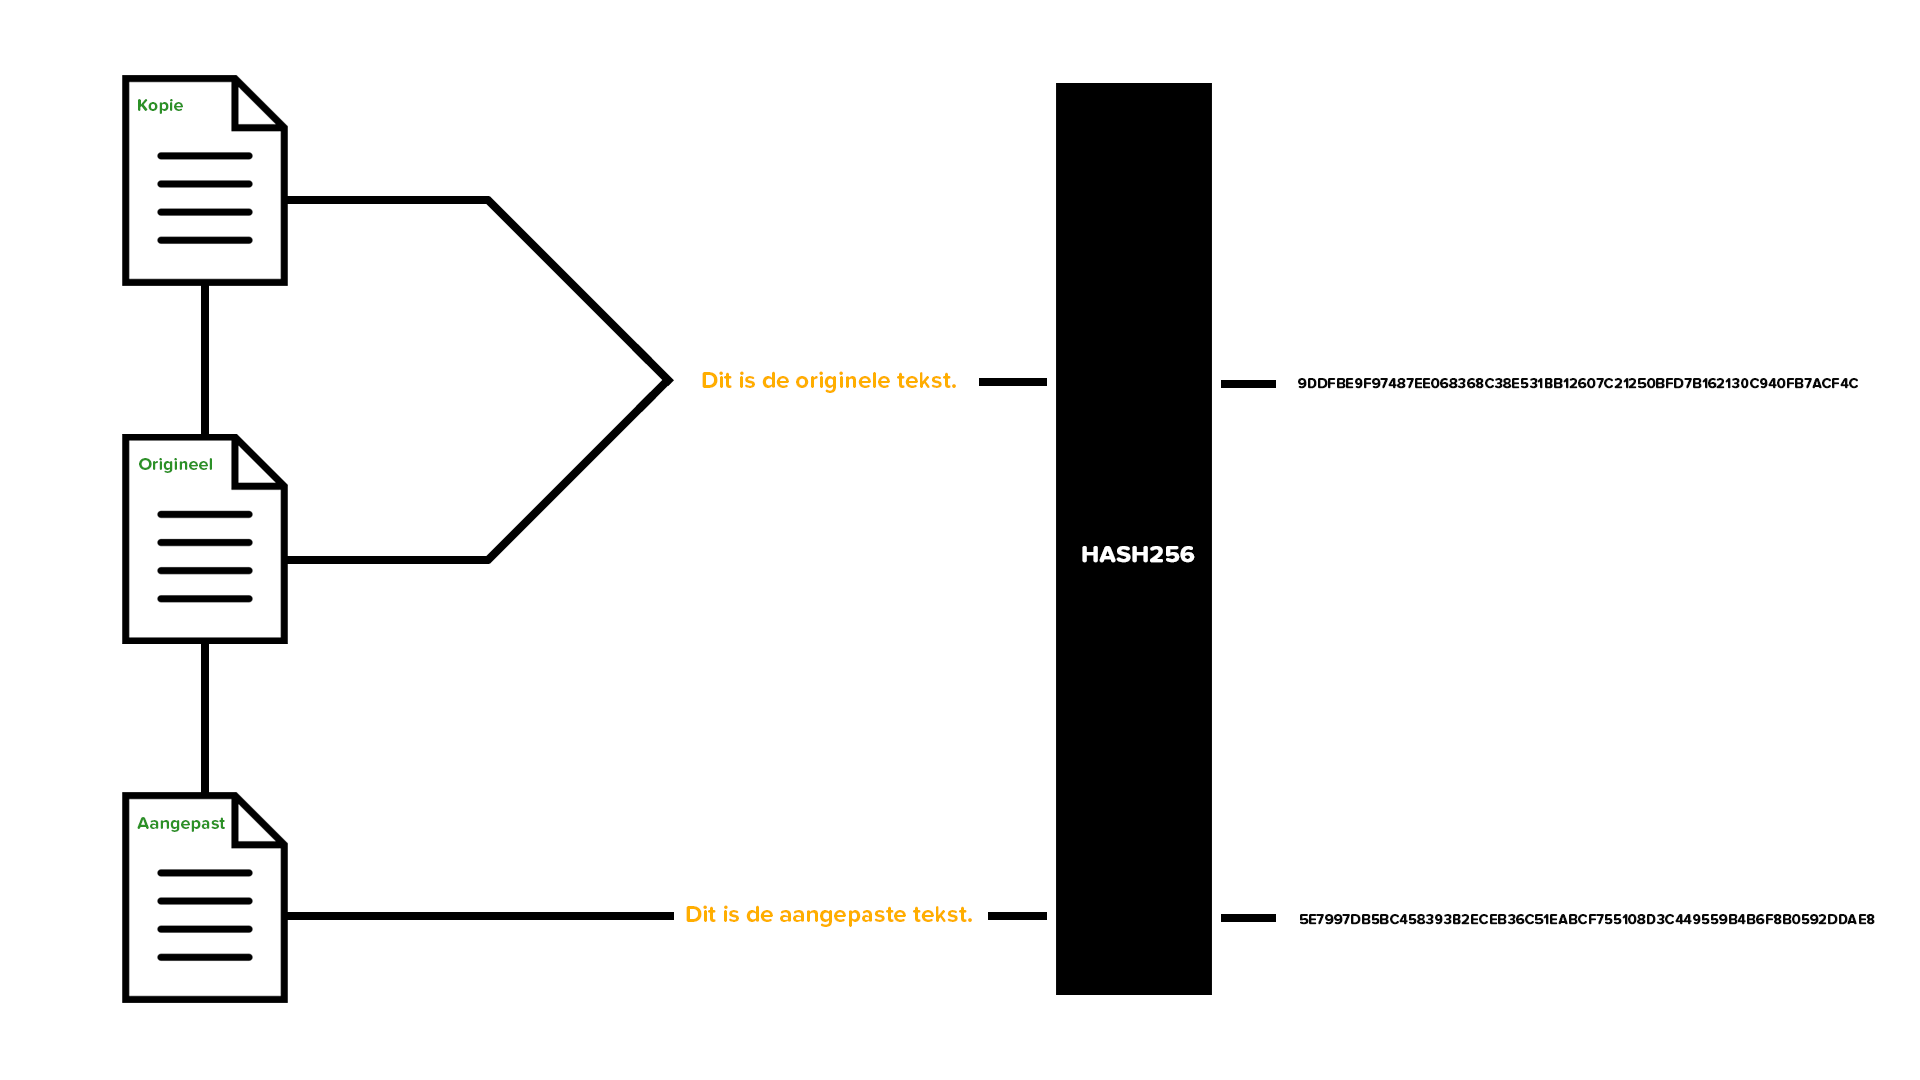
\includegraphics[width=\linewidth]{hash-example.png}
	\caption{Grafische voorstelling van de werking van Sha256.}
	\label{fig:hash-example}
\end{figure}

\section{Algoritmes}
Er zijn verschillende overeenkomst algoritmes die gebruikt worden voor elk type blockchain. Elk type van algoritme kan ook gebruikt worden in andere types van blockchain maar deze zijn niet altijd even effectief en dit wordt hierdoor meestal ook niet gedaan. De volledige opstelling van blockchain is namelijk volledig naar wens in te stellen. Daarom worden er ook vaak enkele types gedefinieerd die verder aan bod komen.

\subsection{Proof-of-work algoritme?}
Proof-of-work is een maatregel die werd ingevoerd om bepaalde aanvallen te voorkomen zoals de gekende denial of service of ook DOS-aanvallen genoemd of om spam op een publiek netwerk tegen te gaan en dit door werk te vragen van de service aanvrager meestal in de vorm van verwerkingstijd door een computer. Proof-of-work kan voorkomen in verschillende vormen, meestal zijn dit wiskundige algoritmen. Enkele voorbeelden zijn puzzels, Diffie-Hellman puzzels, hash sequencies, Merkle tree gebaseerde algoritmen en nog enkele meer. 

Verder zijn er ook verschillende varianten. Deze zijn de Challenge-response en Solution-verification. Het verschil tussen beide kort samengevat komt neer op het volgende, bij challenge-response is de taak die moet uitgevoerd worden nog niet bekend. De server zal deze sturen bij het aanvragen van een service. Bij Solution-verification is de taak op voorhand gekend en kan deze meteen meegestuurd worden met de request \textcite{Mazieres}. De proof-of-work die Bitcoin zelf gebruikt is bijvoorbeeld gebaseerd op Adam Back's Hashcash \textcite{Nakamoto2008}.

Proof-of-work wordt vooral gebruikt in een publiek netwerk waar geen rechten van toepassing zijn. Iedereen heeft dus evenveel inspraak. Voor andere types van blockchain is dit weer minder van toepassing aangezien de werking niet optimaal zou verlopen. Wanneer men bijvoorbeeld proof-of-work zou gebruiken in een privé netwerk waar alle nodes gekend zijn dan is er weinig nut tot het gebruiken van proof-of-work. Als iemand een aanval probeert te doen op het netwerk dan kan er snel aangewezen worden wie de schuldige was. Proof-of-work zou het geheel ook alleen maar vertragen aangezien er in dit geval telkens een proof-of-work gegenereerd zou moeten worden en dit tijd en CPU-kracht kost. 

\begin{figure}
	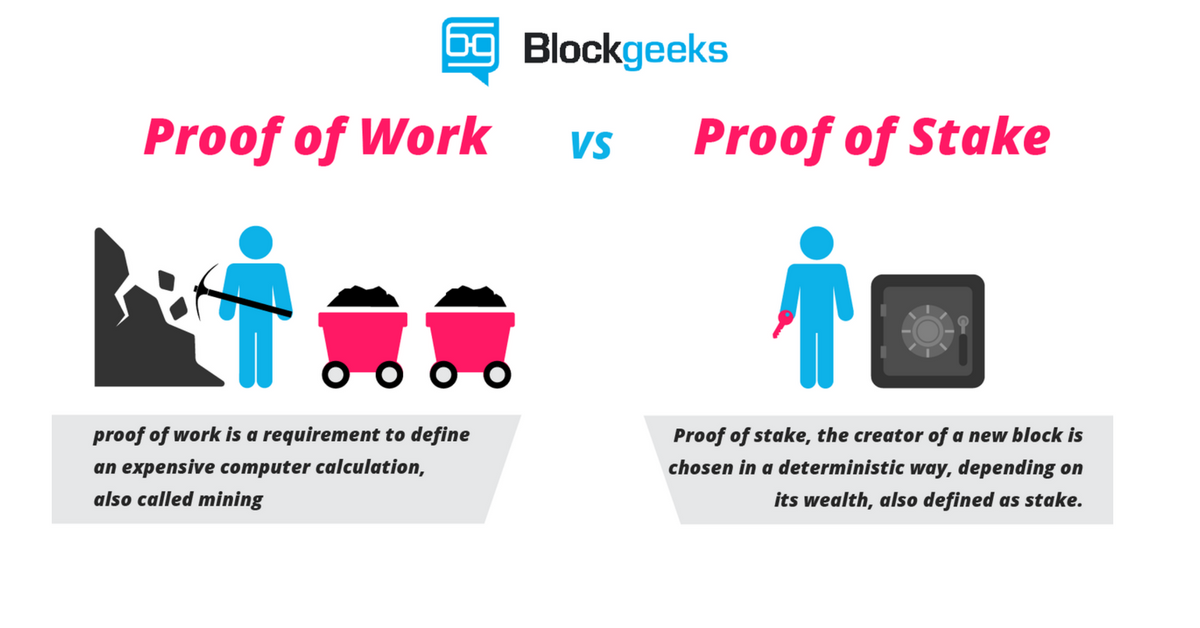
\includegraphics[width=\linewidth]{pow-vs-pos.png}
	\caption{Grafische voorstelling van proof of work tegenover proof of stake \textcite{blockgeeks}.}
	\label{fig:pow-vs-pos}
\end{figure}

\subsection{Proof of stake algoritme}
Wanneer er proof of stake gebruikt wordt om een overeenkomst te bekomen dan wordt er meteen ook vanuit gegaan dat elke node niet meer dezelfde rechten heeft, niet iedereen heeft dus evenveel inspraak meer. Proof of stake werkt volgens het principe dat iemand met meer ``aandelen'' in het netwerk dus ook meer inspraak heeft. Dit heeft als voordeel dat iemand met veel aandelen dus het netwerk niet zal proberen bedriegen aangezien hij deze anders verliest. Het is dus met andere woorden niet de moeite om het netwerk op te lichten en iemand met weinig inspraak of ``aandelen'' heeft ook weer niet genoeg inspraak om het systeem op te lichten. Iemand met veel aandelen zal dus grotere kans hebben om een nieuw blok aan te maken dan iemand met een kleiner aandeel \textcite{Buterin2013}. In Figuur \ref{fig:pow-vs-pos} is een grafisch voorbeeld tussen proof of work en proof of stake te zien.

\subsection{Federated Byzantine Agreement algoritme}
Dit is een methode van overeenkomst die ook gebruik wordt in publieke omgevingen zonder rechten. Natuurlijk moet er ook kunnen getolereerd worden dat er mag gelogen worden of verkeerde informatie mag verzonden worden. Dit noemt met ook wel Byzantine failure. Het is dus vooral belangrijk dat er een overeenkomst tot stand komt ook al werken alle nodes onafhankelijk van elkaar. Er zijn enkele verschillen tussen een Byzantine agreement en een federated Byzantine agreement, het grootste verschil is alvast dat bij een Byzantine agreement alle nodes unaniem moeten overeenkomen. Dit is bij een federated Byzantine agreement anders. Zo kiest hier elke node zelf welke node er vertrouwd wordt en welke niet. Er is dus geen centrale authoriteit gemoeid in het systeem. Nodes kunnen bijvoorbeeld nodes vertrouwen op basis van criteria. Bijvoorbeeld een bank zou als vertrouwbaar kunnen gezien worden, op deze manier kunnen andere nodes herkenning vragen van alle transacties aan deze node. Meestal worden de groeperingen van de nodes overlapt zodat er altijd een algemeen besluit is. Wanneer de nodes niet zouden overlappen dan zou groep 1 van nodes kunnen kiezen voor het ene waar groep 2 zou kunnen kiezen voor het andere. Daarom wordt meestal gebruik gemaakt van een overlapping.

\subsection{Quorum}
Er zijn verschillende manieren mogelijk van indelen, disjuncte groepen en groepen met een intersectie. Voordelig is om toch een intersectie groep te gebruiken maar dit kan natuurlijk altijd afhangen van de usecase. Het grote verschil tussen beide wordt weergegeven op deze figuur. Hier zijn  2 groepen te zien zonder een node die ze gemeen hebben samen met een groep waar enkele nodes wel gemeenschappelijk zijn. Op deze manier wordt er altijd een algemeen akkoord bekomen. Dit kan niet altijd het geval zijn in een disjuncte groep aangezien de ene groep optie 1 kan kiezen terwijl de andere optie 2 kan kiezen en er dus geen algemeen akkoord bekomen wordt \textcite{Stellar2015}.

\begin{figure}
	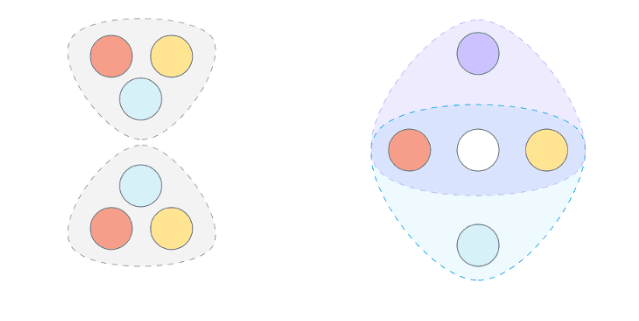
\includegraphics[width=\linewidth]{quorum.png}
	\caption{Een weergave van het verdelen van nodes in groepen \textcite{Stellar2015}.}
	\label{fig:quorum}
\end{figure}

\subsection{Multisignature algoritme}
Als laatste is er multi-sig of multisignature. Deze is er gekomen door één van de problemen die het Bitcoin netwerk tegen kwam en dit was het volgende. Alle bitcoins worden opgeslagen op 1 adres zoals voorheen overlopen, en dit in een wallet. Het nadeel is, iedereen die de privé sleutel heeft tot dit adres heeft ook meteen het recht om transacties uit te voeren en dus het geld over te schrijven. Hierdoor is men opgekomen met multi-sig. Een nieuw type van adres genaamd pay-to-script-hash of afgekort P2SH. Doorheen dit onderwerp wordt dan ook de afkorting gebruiken. Een duidelijk kenmerk van een P2SH adres is dat deze start met een 3. Verder wordt er ook de functionaliteit ondersteund waar er meerdere privé sleutels nodig zijn om een transactie uit te kunnen voeren. Meestal wordt er in de praktijk 2-of-2 of 2-of-3 gebruikt. Dit komt voor bij de werking van een kluis in de bank. De klant heeft hier 1 sleutel en de bank zelf. Dus men heeft beide sleutels nodig om toegang te verkrijgen tot de kluis. Dit komt overeen met een 2-of-2 multi-sig adres. 

Dit heeft meteen ook enkele voordelen wanneer met multi-sig gebruikt. Zo is er geen enkel punt meer van zwakte, hiermee bedoelt men dat wanneer 1 toestel gehackt zou worden dat er nog steeds geen transactie kan plaatsvinden aangezien er een tweede sleutel vereist is. Natuurlijk moet er voor gezorgd worden dat beide sleutels op verschillende toestellen staan en één toestel dus niet beide sleutels heeft. 

\begin{figure}
	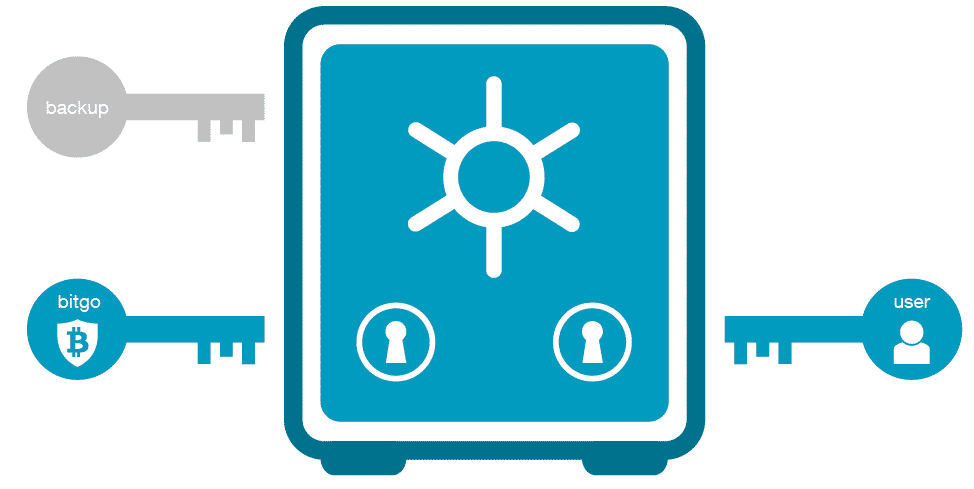
\includegraphics[width=\linewidth]{multisig.png}
	\caption{Een grafische voorstelling van de werking van multi-sig \textcite{99bitcoins}.}
	\label{fig:multisig}
\end{figure}

Stel dat één van de sleutels zich op een mobiel toestel bevindt en men raakt dit toestel kwijt? 
Dan is dit alweer geen probleem wanneer men gebruik maakt van een 2-of-3 opstelling. Dit wil zeggen dat de gebruiker 1 van de sleutels zelfs mag verliezen omdat er 3 sleutels voorzien zijn die kunnen gebruikt worden. Dit zou kunnen betekenen dat de derde sleutel zich bijvoorbeeld offline bevindt in een ``kluis''. Deze voorstelling is te zien op Figuur \ref{fig:multisig}. Deze overeenkomst strategie heeft dus heel wat mogelijkheden en beveiligen ook het netwerk wanneer één node zou gehackt worden dat er aanvallen op het systeem gebeuren en transacties plaatsvinden met slechte intenties. 

\subsection{Round Robin algoritme}
Een ander veel gebruikt algoritme is Round Robin. Dit houdt in dat er willekeurig een node zal worden gekozen. Wanneer een specifieke node gekozen wordt, dan wordt deze uitgesloten van volgende transacties en wordt deze node niet meer toegestaan een blok aan te maken voor een ingesteld aantal transacties. Op deze manier wordt voorkomen dat er voortdurend aanvallen op het netwerk gebeuren aangezien de node willekeurig wordt gekozen. Al wordt een node met slechte bedoelingen gekozen dan zal hij geen poging meer kunnen ondernemen voor de volgende aantal transacties. 

\section{Veiligheid}
Blockchain is uitermate veilig, maar een systeem is uiteraard maar zo sterk als zijn zwakste schakel. Wanneer er dus verkeerd wordt omgegaan met deze technologie kan het dus al snel fout lopen. Dit door bijvoorbeeld fouten in code of het onveilig omgaan met data na dit van de blockchain gehaald te hebben. Er zijn dan ook enkele zaken waar streng opgelet moet worden en rekening mee gehouden moet worden. 

\subsection{Double spending}
\label{sec:hoeveiligisblockchain}
Wanneer er dus een aanval gebeurt op de blockchain of dus een illegale transactie plaats vindt dan kan deze verworpen worden door de andere servers. In simpele termen komt het er op neer dat zolang de totale CPU capaciteit van de servers groter is dan de capaciteit van de aanvaller dat de blockchain dus veilig is en de aanvallen zal afweren. Dit omdat de aanvaller sneller een alternatieve ketting zou moeten produceren  dan dat de vertrouwde nodes dit doen. Zelf in het geval dat dit zou gebeuren wil dit niet zeggen dat de vertrouwde nodes dit zullen accepteren aangezien dat de aanvaller ook geen waarde kan creëren uit het niets of zichzelf eigenaar kan maken van andere waarden als dit zou bekeken worden in het systeem van Bitcoins. Het enige wat een aanvaller dus in principe kan doen is het aanpassen van zijn eigen transacties, bijvoorbeeld dus geld terug nemen dat hij al eerder uitgaf of ook ``double spending'' genoemd. Verder zijn er natuurlijk nog andere mogelijkheden waar er rekening moet mee gehouden worden op vlak van veiligheid. De kans dat zich dit voordoet is uitermate klein. Zo is te zien in de whitepaper van \textcite{Nakamoto2008}. Stel dat de aanvaller 10 blokken achter zit en de vertrouwde ketting moet inhalen dan heeft deze een kans van 0.0000012\% wanneer men er vanuit gaan dat de aanvaller 10 \% kans heeft om de volgende blok te vinden. Verdere berekeningen zijn te vinden in de paper van \autocite{Nakamoto2008}.

\subsection{Andere soorten ``hacks''}
Er zijn uiteraard verschillende manieren van ``hacken'', één van de bekendste is bitcoin mining malware. Dit is malware die verspreid wordt en computers en apparaten infecteert. De geïnfecteerde apparaten worden hierdoor gebruikt om bitcoins te minen wat de toestellen uiteraard zwaar vertragen. 

Andere zaken die veel voorkomen zijn het hacken van de bitcoin wallets, dit zijn bestanden die op de machine staan en die de bitcoins bijhouden. Deze ``wallets'' bevinden zich op de hardeschijf en kunnen dus gestolen worden. 

Trojans zijn ook bij bitcoin een plaag. Zo zijn er trojans die slechts activeren wanneer er een crypto-currency nummer wordt ontvangen en die deze dan manipuleren zodat de gebruiker bijvoorbeeld geld overschrijft naar de verkeerde persoon. 

Verder zijn er ook nog fouten in de software die bijvoorbeeld toegang geeft tot een blockchain. Blockchain mag in theorie en praktijk nog zo veilig zijn, als er software gebruikt wordt die malfunctioneert dan kan de veiligheid van blockchain ook snel te niet gedaan worden.

Zoals eerder vermeld zijn de transacties of sommige zaken versleuteld voor het publiek. De transactie zelf is zichtbaar maar sommige zaken zijn versleuteld. Wanneer deze encryptie bijvoorbeeld niet sterk genoeg is kan het zijn dat hackers een bepaald deel van de versleutelde tekst toch kan ontfutselen. Blockchain gebruikt in het algemeen een Sha-256 versleuteling, deze wordt onder andere ook gebruikt voor het versleutelen van HTTPS en dergelijke. Wanneer deze encryptie zou falen zou niet enkel blockchain dus een zwaar probleem hebben. Onderzoek bevestigde wel dat Sha-256 zeker sterk genoeg is om zaken te beveiligen voor een hele tijd wanneer dit op een goede manier gebruikt word. Zo heeft Bitcoin enkele strenge eisen voor een geldige hash \textcite{Faife2017}.

\section{Automatisering}
Op sommige systemen is zelf rekening gehouden met automatisering. Zo is het bijvoorbeeld mogelijk om bepaalde taken automatisch te laten gebeuren wanneer er aan bepaalde criteria wordt voldaan. Een goed voorbeeld hiervan zijn smart contracts.

\subsection{Smart contracts}
Smart contracts zijn computer protocols die bedoeld zijn om het toepassen van een contract te vereenvoudigen en te verifiëren. De bedoeling van smart contracts is om bepaalde zaken te kunnen coderen die dan later automatisch kunnen uitgevoerd worden. Een grafisch voorbeeld is te vinden in Figuur \ref{fig:smartcontracts}. De scripts zijn vooral populair op de Ethereum blockchain (een andere cryptocurrency) en worden hier ook wel dapps genoemd of decentralised applications. Een populaire programmeertaal voor het maken van smart contracts is dan ook ``Solidity''. Deze scripts worden dan opgeslagen in de blockchain zodat ze later kunnen uitgevoerd worden door de EVM (Ethereum Virtual Machine)  \textcite{Chandrayan2017}.

\begin{figure}
	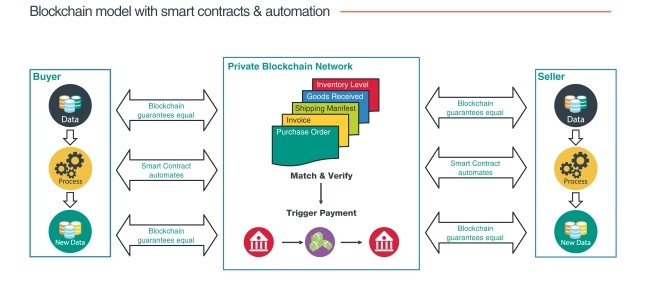
\includegraphics[width=\linewidth]{smartcontracts.jpeg}
	\caption{Grafische voorstelling van de werking van smart contracts  \textcite{Itweb}}
	\label{fig:smartcontracts}
\end{figure}

%%\lipsum[7-20]

%%=============================================================================
%% Verzekeringen
%%=============================================================================

\chapter{Verzekeringen}
\label{ch:insurance}
\section{Verzekeringsagenten, wat doen ze en waar komen ze vandaan?}
Een verzekeringsagent is een gebonden tussenpersoon. Dit wil zeggen dat deze persoon voor één verzekeringsmaatschappij werkt, dit verschilt van een verzekeringsmakelaar die onafhankelijk is en niet gebonden is aan één verzekeringsmaatschappij. Een verzekeringsagent kan dus slechts de verzekeringen aanbieden van zijn eigen maatschapij waar een verzekeringsmakelaar verzekeringen kan aanbieden van verschillende maatschapijen. 

Er zijn uiteraard meerdere benamingen voor een verzekeringsagent die allemaal op hetzelfde neerkomen zo wordt een verzekeringsagent bijvoorbeeld ook een tussenpersoon genoemd, een intermediair of een financieel adviseur.

\section{Verzekeringen en unieke documenten}
Een verzekeringsagent en verzekeringsmakelaar doen dus juist hetzelfde. Het enige verschil tussen beide is dus dat een verzekeringsagent gebonden is aan één maatschapij waar een verzekeringsmakelaar dit niet is. Voor vereenvoudiging doorheen dit document zal ik steeds verwijzen naar een verzekeringsmakelaar. 

Wat doet een verzekeringsmakelaar nu juist? Een verzekeringsmakelaar zal jouw wensen en vragen allemaal noteren en zal dit gebruiken om de voor u zo optimale verzekering te vinden. Nadien overloopt deze dan alle mogelijkheden met de nodige uitleg. Verzekeren kan een zeer complex iets zijn en dan is een verzekeringsmakelaar zeker nuttig om te raadplegen  \textcite{Verzekeruzelf.nl}.

\subsection{Soorten verzekeringen en verzekeringsdocumenten}
Er zijn heel veel soorten verzekeringen. Zo kan in theorie alles verzekerd worden al is dit niet altijd gebruikelijk. In volgend document \textcite{verzekeringen.com2015} zijn enkele voorbeelden van beroemdheden die verschillende lichaamsdelen lieten verzekeren te vinden want ook dit is uiteraard mogelijk. Bijvoorbeeld wanneer een gitarist zijn hand zou verliezen dan verliest deze hiermee ook meteen de mogelijkheid tot het uitoefenen van zijn beroep. Er zijn dus heel wat mogelijkheden beschikbaar, volgens het volgende artikel \textcite{BFOverzekeringen} van de Belgische overheid zijn dit de meest voorkomende verzekeringen.

\begin{itemize}
	\item Autoverzekering
	\item Brandverzekering en natuurrampen
	\item Familiale BA-verzekering
	\item Rechtsbijstand
	\item Ziekte- en hospitalisatieverzekering
	\item Reisverzekering
	\item Vrijwilligersverzekering
	\item Schuldsaldoverzekering
	\item Levensverzekering of overlijdensverzekering
	\item Verzekeringen in specifieke situaties
\end{itemize}

Voor elk van bovenstaande verzekeringen is er dus een contract, dit bijgevolg ook uniek zal zijn en bepaalde voorwaarden zal bevatten. Documenten zoals deze zouden dus perfect in een blockchain kunnen opgeslagen kunnen worden. 

\section{Is verzekeren verplicht?}
Er wordt inderdaad ook onderscheid gemaakt tussen verplichte verzekeringen en niet verplichte verzekeringen. Zo kan men verplicht zijn een verzekering te nemen om een bepaalde activiteit te mogen uitvoeren. Denk maar aan een BA verzekering, wanneer een wagen niet verzekerd is dan kan deze niet in verkeer worden gebracht. Daar tegenover is een bestuurdersverzekering geen verplichte verzekering. Ook voor het uitvoeren van bepaalde beroepen is het verplicht om een verzekering aan te gaan. Enkele voorbeelden zijn architecten, boekhouders, belastingsconsulenten en nog vele meer. Sommige verzekeringen kunnen dan weer wel contractueel verplicht worden. Zo kan een huisbaas bijvoorbeeld de huurder verplichten een brandverzekering af te sluiten  \textcite{BFOverplichteVerzekeringen}. 

\chapter{Data en de blockchain}
\label{ch:add-to-blockchain}

\section{Introductie}
Het toevoegen van data gebeurt door het uitvoeren van transacties. De transacties worden vervolgens in een blok geplaatst en verzonden over het netwerk naar elke node om deze transactie te verifiëren. Elke node werkt onafhankelijk en zal het blok voor zichzelf valideren of weigeren. Wanneer een blok gevalideerd wordt door een node zal deze het geverifieerde blok terug verzenden naar alle nodes op het netwerk om dit ook aan de andere nodes te laten weten. Hoe men de transactie valideert is door een voorafgekend algoritme toe te passen op de hash. 

\section{Overeenkomst tussen nodes}
Elke node valideert dus voor zichzelf of een bepaalde transactie correct is. Er moet uiteraard ook gecommuniceerd worden tussen de nodes om tot een akkoord te komen. Dit zal afhangen van het elk type blockchain die gebruikt zal worden om het meest ideaale resultaat te bekomen. In theorie kan elk algoritme gebruikt worden in elk type blockchain maar dit is niet aan te raden. Om een voorbeeld te geven is het niet gunstig om ``proof of work'' te gebruiken in een privé netwerk met gekende nodes aangezien dit veel trager zal werken.

\section{Welke data wordt toegevoegd?}
Voornamelijk zullen er steeds documenten worden toegevoegd aan de blockchain. Bovendien is het ons doel om alle communicatie te laten verlopen via de blockchain zodat er geen communicatie vereist is buiten het systeem. Op deze manier wordt er een centraal eco-systeem opgebouwd dat alle data bevat.

\subsection{Beveiligen van documenten}
Om te beginnen zal de verzekeringsagent het document moeten aanmaken en in orde maken zodat deze alle nodige gegevens bevat. Verder kan dit document met software versleuteld worden door Sha256 zodat dit document verder niet meer leesbaar is. Dit document kan vervolgens verstuurd worden naar alle andere nodes om dit document te valideren. Aangezien een verzekeraar ook steeds werkt met gevoelige data zal steeds alle data versleuteld worden. 

\subsubsection{Soorten beveiligingen}
Er zijn uiteraard nog andere soorten beveiligingen beschikbaar dan Sha256 zoals Sha384, Sha512 en nog vele meer. Momenteel is er heel wat rekenkracht nodig om Sha256 te breken en dit zou heel wat tijd in beslag nemen dus voorlopig is Sha256 voldoende veilig. Hierdoor zal het encoderen van de bestanden steeds gebeuren met Sha256 maar moet er in gedachten worden gehouden dat dit algoritme ooit gebroken zal kunnen worden en dat er zal moeten overgestapt worden naar een meer complex algoritme zoals Sha384. 

\chapter{Het eco-systeem}
\label{ch:eco-system}
Door gebruik van enkele usecases tonen we aan waarom een centraal eco-systeem in blockchain handig en krachtig zou zijn voor alle partijen. Enkele zaken moeten beslist worden op voorhand. 

\begin{itemize}
	\item Welk type blockchain gaan we gebruiken?
	\item Heeft elke node even veel inspraak?
\end{itemize}

\section{Publieke blockchain}
Wanneer er  gewerkt met een publieke blockchain die toegangelijk is voor iedereen kan er meteen onderscheid gemaakt worden tussen het toepassen van regels of te werken met een systeem zonder regels. Hiermee wordt bedoeld of de ene node evenveel zeggenschap heeft als een andere willekeurige node. Aangezien dit systeem vooral bedoeld is voor het optimaliseren van het hele systeem kan dit wel gebruikt worden maar zullen er toch enkele zaken moeten aangepast worden.

\subsection{Proof of work}
Iedereen in een publiek netwerk is namelijk niet gekend. Men weet dus niet wie een transactie start of valideert of dergelijke. Niemand beheert het systeem dan ook aangezien elke node dezelfde inspraak heeft. Ook zal een publiek systeem zonder regels moeten werken aan de hand van een proof of work systeem wat dus bij elke transactie rekenkracht van de CPU zal vereisen van de nodes. Dit neemt meteen ook tijd in beslag, het hele systeem wordt dus minder performant. Het gebruik van een systeem waar iedereen dezelfde inspraak heeft lijkt dus al meteen een minder goede keuze. Verder heeft dit ook het nadeel dat er hoge transactie kosten zullen opduiken door het gebruik van een publiek netwerk. Een voordeel hieraan is natuurlijk dat er gebruik kan gemaakt worden van een bestaand netwerk en er zelf geen systeem moet opgesteld worden. 

\subsection{Proof of stake}
Aangezien er toch enkele grote partijen mee gemoeid zijn, zullen die meteen ook te vertrouwen zijn is het ook geen slecht idee om te werken met proof of stake en toch enkele nodes meer recht te geven dan andere. Zo zal een verzekeringsmaatschappij bijvoorbeeld veel documenten beheren en aanmaken en hierdoor dus ook meer inspraak hebben in het systeem. Dit lijkt ook logischer dan wanneer elke node even veel inspraak heeft aangezien er toch enkele gekende partijen bij betrokken worden. Dit biedt ook meteen voldoende veiligheid aangezien verzekeringsmaatschappijen geen aanvallen en dergelijke zullen verrichten op het netwerk dit zou ook meteen strafbaar zijn. Natuurlijk blijven de hoge transactie-kosten toch nog steeds een klein minpuntje waar de terug verkregen performantie door gebruik van proof of stake een pluspunt is. 

\subsection{Smart contracting}
Wanneer er gebruik wordt gemaakt van een platform zoals Ethereum dan kan men ook gebruik maken van smart contracts. Een heel groot deel kan dus geautomatiseerd worden, bijvoorbeeld er gebeurt een ongeval, een cliënt laadt het schadeformulier op. Hier kan smart contracting gebruikt worden om een hele boel te automatiseren. Dit kan al meteen het probleem oplossen dat een cliënt nooit weet hoever zijn schadedossier staat. Bij elke stap die wordt uitgevoerd kan er bijvoorbeeld automatisch een service aangesproken worden die de cliënt automatisch op de hoogte houdt van de stand van zaken. Bijvoorbeeld wanneer de verzekeraars contact opnemen met elkaar, wanneer er contact is opgenomen met de partij die het schadegeval zal komen waarnemen, wanneer de schaderaming is ontvangen en nog zo veel meer. 

\section{Privé blockchain}
Waar een publieke blockchain totale anonimiteit biedt zal een privé blockchain weten welke node wat heeft gedaan. Dit is ook meteen een veiligere omgeving aangezien alle nodes gekend zullen zijn. Dit is natuurlijk een pluspunt aangezien er gewerkt wordt met gevoelige informatie die niet voor iedereen bedoeld is. Aangezien er enkele partijen mee gemoeid zijn is het ook geen slechte keuze aangezien elke partij een node kan zijn. Een ander pluspunt is dat er geen proof of work meer moet gegenereerd worden en dus het syteem terug een stuk performanter wordt. Een nadeel is natuurlijk dat alle transacties door 1 partij worden beheerd. Bijvoorbeeld de overheid. Alle transacties zullen dus naar deze partij worden gestuurd voor goedkeuring en deze zal dus altijd het nieuwe blok aanmaken. Dit is uiteraard een minder gedecentraliseerd systeem en lijkt meer op een databank met extra beveiliging. 

\section{Consortium blockchain}
Consortium is een type blockchain dat tussen een publiek en een privé netwerk valt. Het netwerk is publiek maar heeft enkele instanties die gekend zijn en die het netwerk volledig beheren. Deze instanties staan ook toe wie de blockchain kan lezen en wie niet. Het hele systeem kan gezien worden als een ``raad der wijzen''. Het voordeel aan het gebruiken van een consortium blockchain is dat het niet beheerd wordt door 1 partij zoals bij een privé netwerk maar door een verzameling van partijen. 

\subsection{Multi-sig}
Het algoritme dat het meest voor de hand ligt in dit geval is Multi-sig. Verschillende partijen hebben elk een sleutel. Zo kan bijvoorbeeld de overheid zelf een sleutel hebben en heeft een verzekeringsmaatschappij een sleutel. Op deze manier moeten er telkens 2 instanties goedkeuring geven aan een transactie waarvan één de overheid zelf is, uiteraard afhankelijk van de opstelling van multi-sig. In het algemeen wordt er gebruik gemaakt van een 2-of-3 opstelling. De reserve sleutel wordt dan ook opgeborgen op een offline locatie voor de veiligheid. Op deze manier is het systeem veilig tegen double spending aanvallen en dergelijke aangezien de overheid zelf telkens goedkeuring moet geven. Dus zelfs al wordt 1 partij gehackt dan zal de transactie nog steeds niet worden goedgekeurd. 

\chapter{Usecases}
\label{ch:usecases}
In dit hoofdstuk zullen er enkele usecases opgesteld en opgelost aan de hand van blockchain. Zo wordt ook meteen het hele eco-systeem getest en kan er nadien een goede conclusie worden gemaakt.

\section{Tekenen van een contract}
De cliënt wil een contract aangaan met een verzekeraar voor het verzekeren van enkele zaken. Hiervoor maakt de verzekeringsagent een contract op dat voldoet aan de eisen van zijn cliënt. Het contract wordt op de blockchain geplaatst als een transactie en zal vervolgens over het Ethereum netwerk worden gebroadcast. Elke node op het netwerk zal vervolgens het document verifiëren, bij validatie zal de transactie worden toegevoegd aan een blok. 

\begin{figure}
	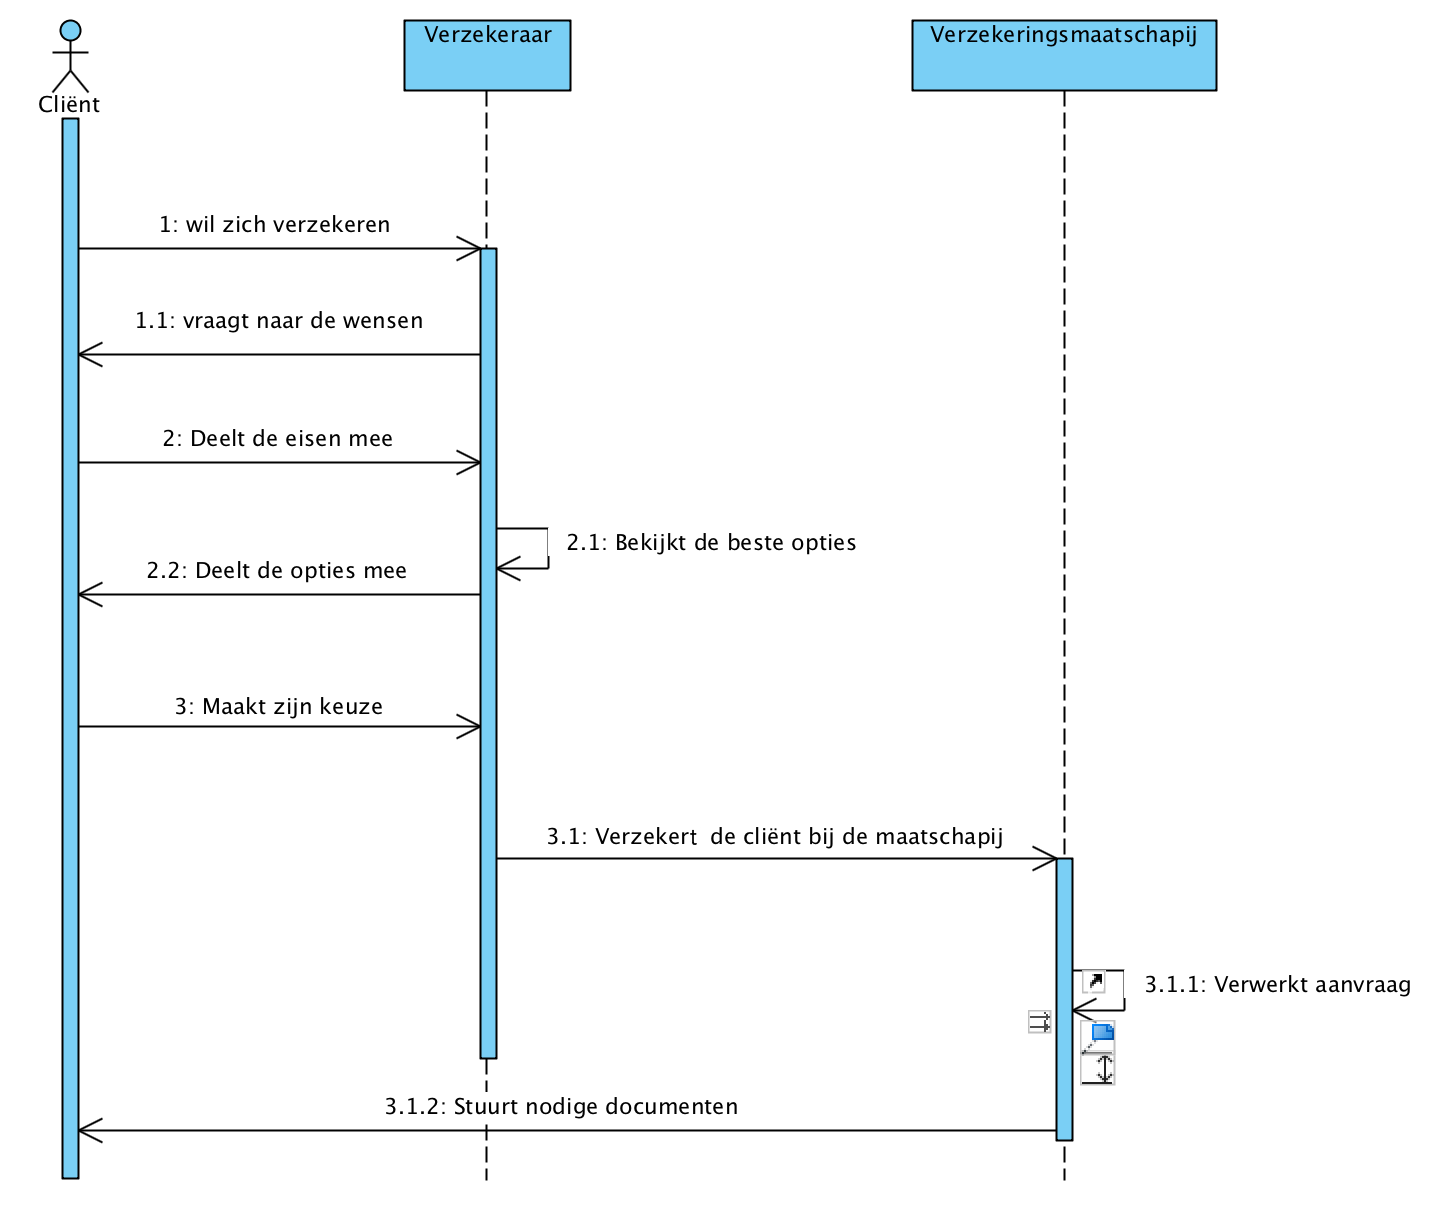
\includegraphics[width=\linewidth]{sd-signcontract.png}
	\caption{Een sequentie diagram die de communicatie aantoont bij het tekenen van een contract. }
	\label{fig:signcontract}
\end{figure}

Vroeger zou dit allemaal moeten gebeuren op kantoor waar beide personen aanwezig moeten zijn. Aangezien dit contract ook zal moeten ondertekend worden ter goedkeuring van de cliënt. Een voorbeeld verloop is te zien op Figuur \ref{fig:signcontract}.

De verzekeraar zou een online platform kunnen maken dat toelaat dat een cliënt zich aanmeldt en een overzicht te zien krijgt van al zijn contracten. Wanneer het contract aan de blockchain werd toegevoegd kan dit ook terug uit de blockchain worden gehaald aan de hand van een versleuteld veld dat uniek is voor deze persoon. Hiervoor zou het rijksregister nummer kunnen gebruikt worden. 

De cliënt krijgt op zijn beurt alle documenten te zien die voor hem bestemd zijn. Dit kan heel groot bekeken worden en kan zelfs verder gaan dan verzekeringsmaatschappij gebonden. Denk maar aan een blockchain die alle verzekeringsdocumenten bevat van een land of continent!

De klant kan vervolgens via dit platform het gewenste document selecteren en tekenen. De handtekening van de klant kan gebeuren aan de hand van een EID lezer zodat deze zijn identiteit moet bevestigen om het document te kunnen tekenen. Dit is uiteraard één van de voorwaarden die moet voldaan worden en waar controle kan naar gedaan worden aangezien dit ook kan toegevoegd worden in de transactie. 

\begin{figure}
	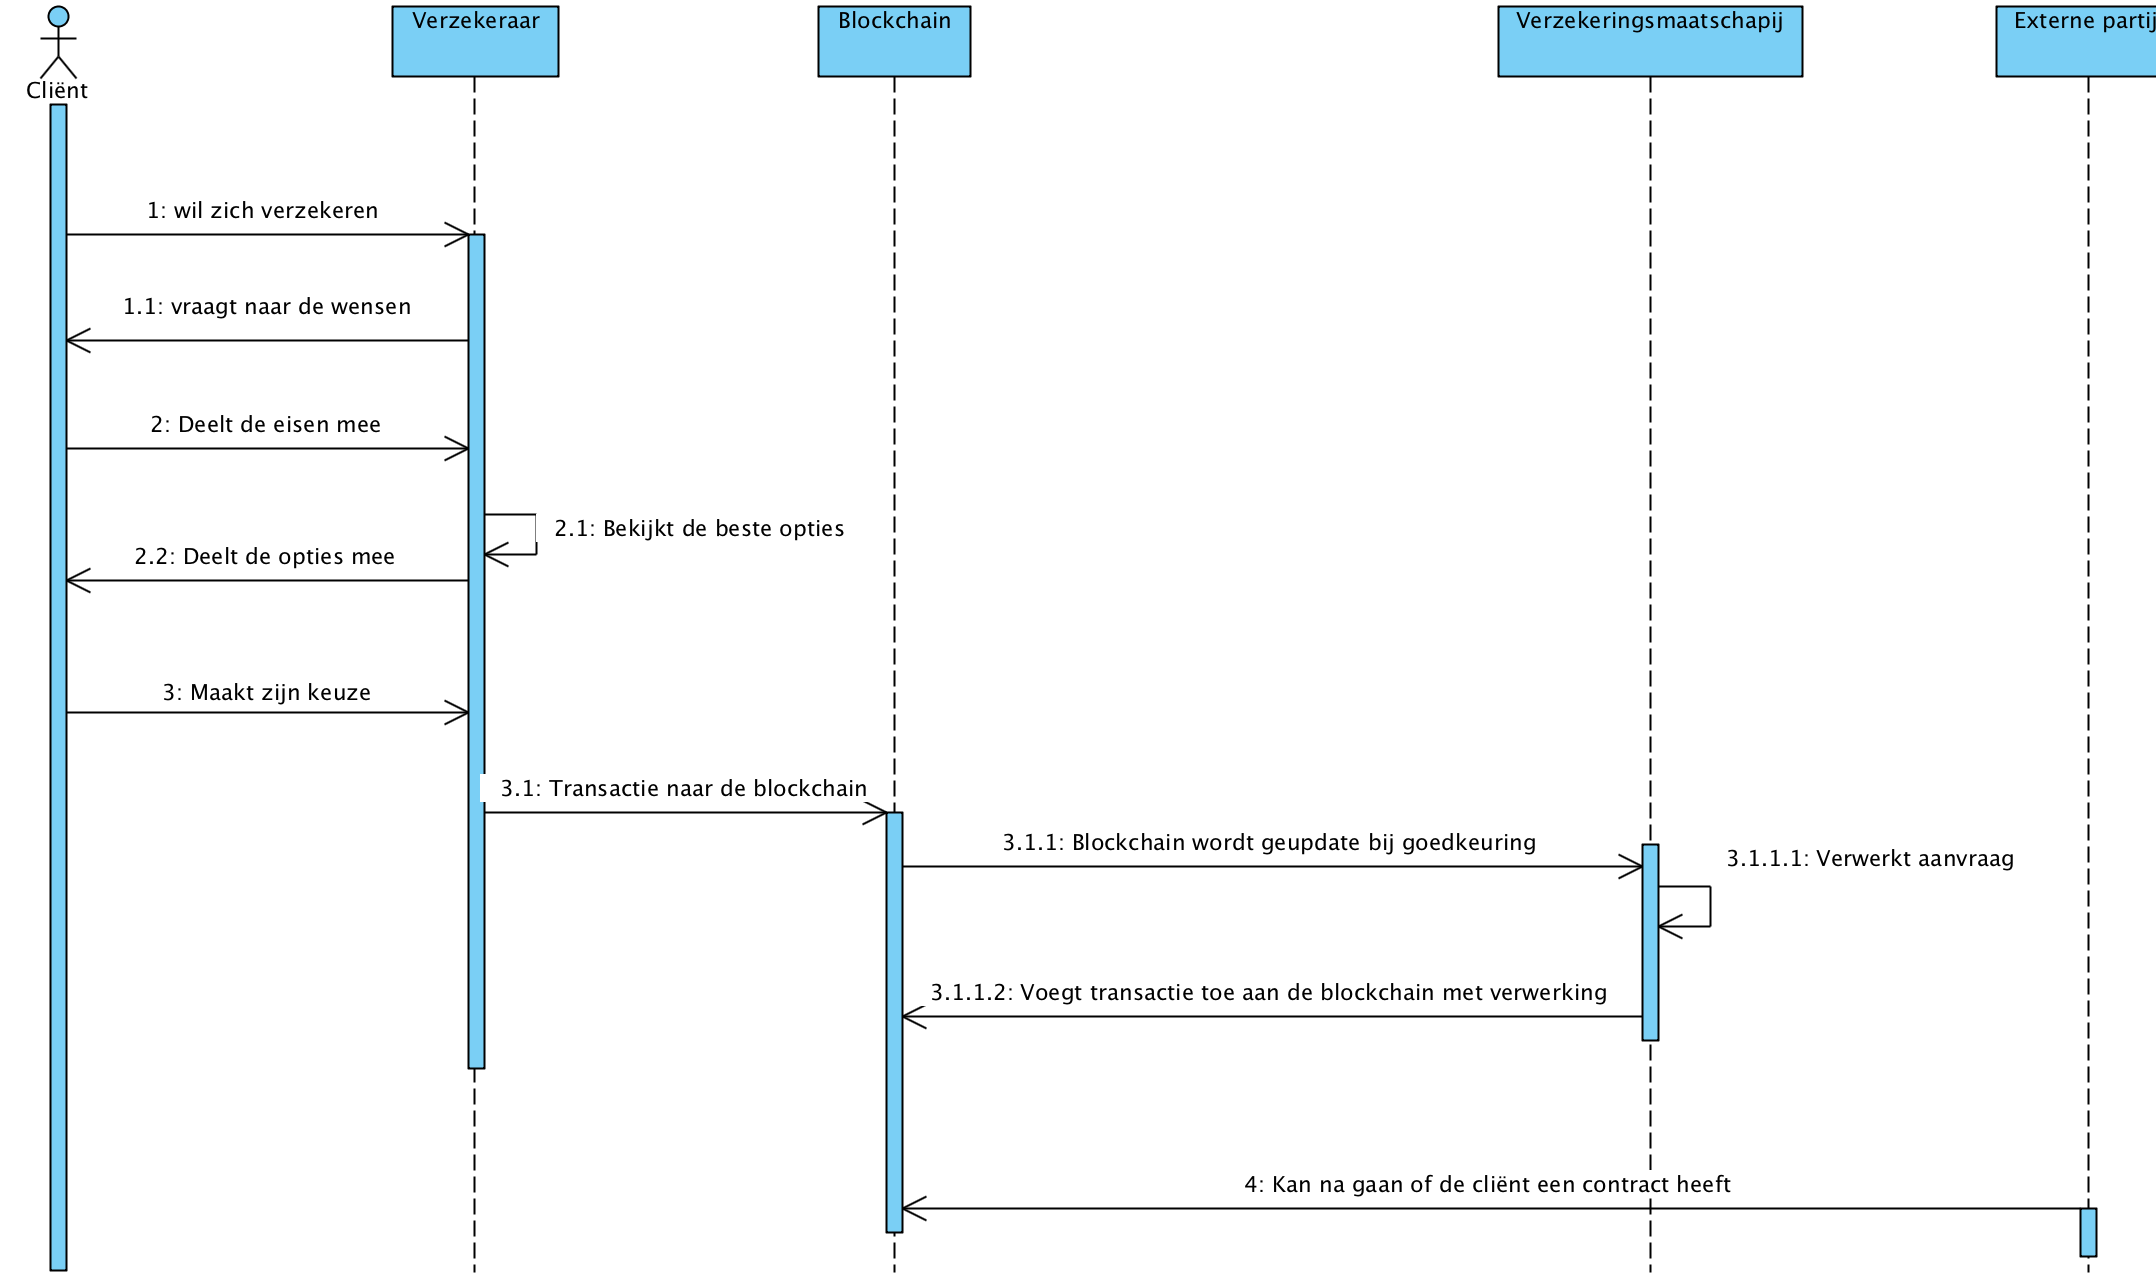
\includegraphics[width=\linewidth]{sd-signcontract-blockchain.png}
	\caption{Een sequentie diagram dat aantoont hoe de communicatie verloopt bij het gebruik van blockchain. }
	\label{fig:signcontract-blockchain}
\end{figure}

Vervolgens zal het webplatform deze handtekening digitaliseren en deze versleutelen. Nadien wordt deze transactie verzonden naar alle nodes om deze te laten verifiëren door het netwerk . Het webplatform is uiteraard ook deel van de nodes in het netwerk om deze verrichtingen te kunnen uitvoeren.

Eenmaal de transactie goedgekeurd werd door het netwerk wordt deze aan het blok toegevoegd. Op deze manier is dit ook zichtbaar voor elke partij dat het contract werd goedgekeurd. 

De cliënt kan dus zijn contracten van thuis digitaal tekenen en op dit moment is dit ook meteen geweten door de andere nodige instanties. Er zijn verschillende opstellingen mogelijk. Een visuele weergave is te zien op Figuur \ref{fig:signcontract-blockchain}.

\section{Aangifte van een ongeval}
Bij een ongeval moet men een schadeformulier indienen, dit wordt ingevuld door beide partijen die betrokken waren bij het ongeval of meerdere partijen indien het gaat om een grootschalig ongeval. Uiteindelijk moet elke betrokkene dit op zijn beurt ook aangeven bij zijn verzekeringsmaatschappij. Vanaf hier wordt alles intern uitgewerkt tussen de verzekeringsmaatschappij die elkaar moeten contacteren, vervolgens nog een partij moet contacteren om de schade van de voertuigen op te nemen en tenslotte te bekijken welke partij in fout gesteld wordt. Een voorbeeld verloop is te zien op Figuur \ref{fig:accident}.

\begin{figure}
	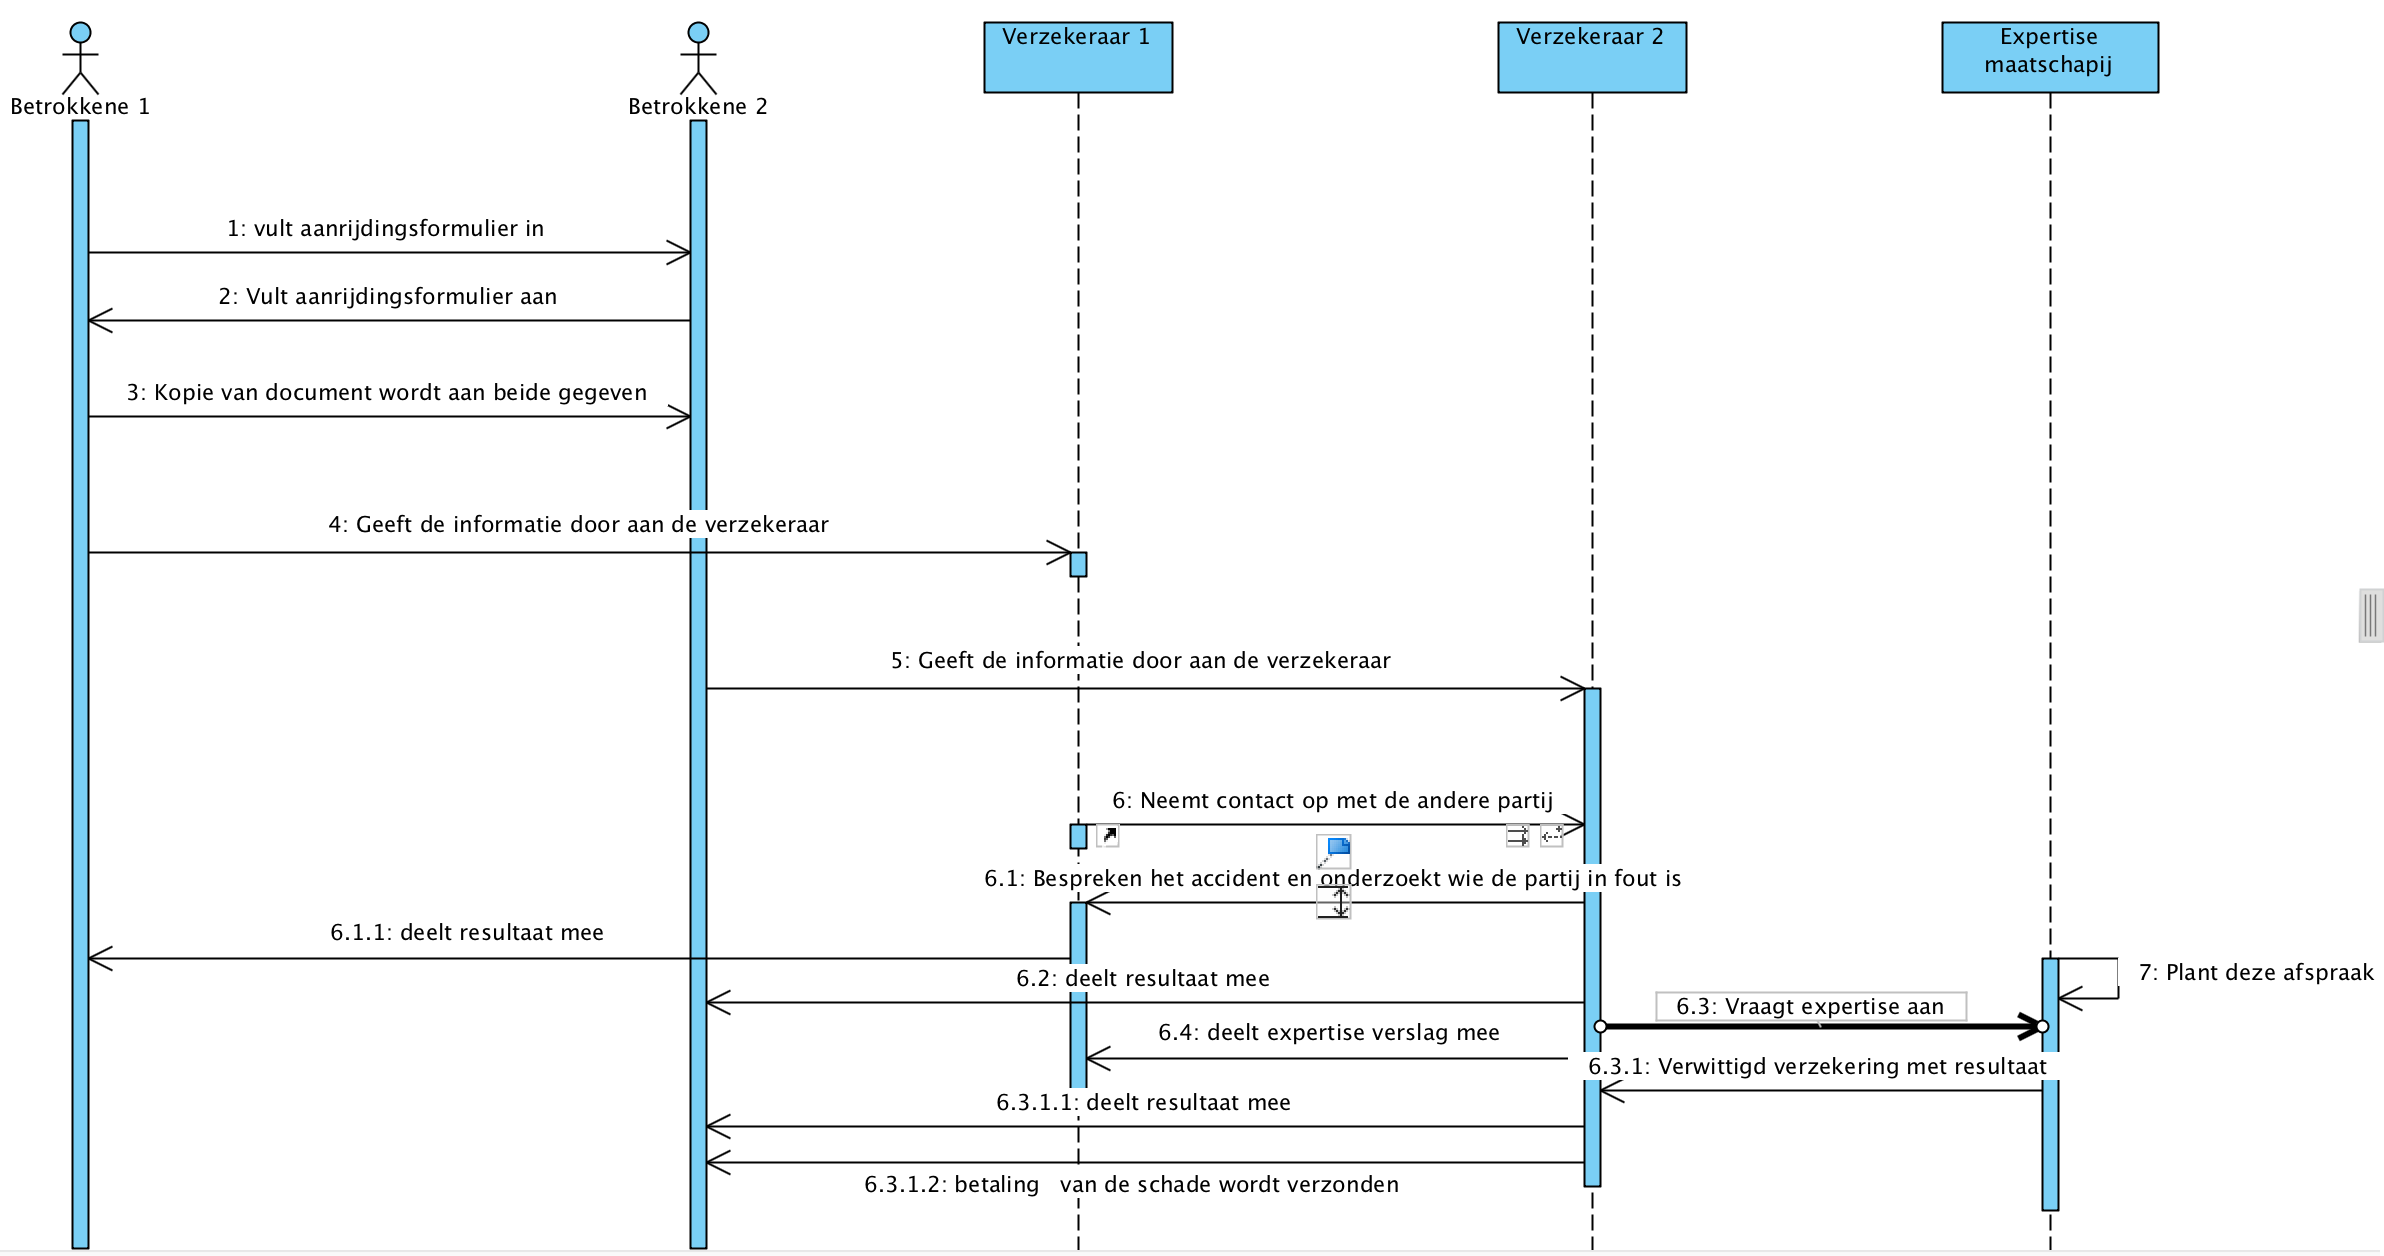
\includegraphics[width=\linewidth]{sd-ongeluk.png}
	\caption{Een sequentie diagram dat de communicatie aantoont tussen verschillende partijen bij een auto ongeluk.}
	\label{fig:accident}
\end{figure}

Ook deze usecase is perfect uit te werken met blockchain. Iedere betrokkene dient zijn formulier in. Dit wordt vervolgens gevalideerd door het netwerk en toegevoegd aan een blok. Hiervoor is natuurlijk vereist dat deze personen ook toegang hebben tot de blockchain. Een platform is dus in dit geval nodig. Een andere oplossing is om de aangifte zelf nog via de verzekeraar aan te geven. Deze kan dan vervolgens de aangifte toevoegen aan de blockchain. Een methode van validatie is ook meteen wanneer alle andere partijen hetzelfde document toevoegen aan de blockchain. Het is ook meteen mogelijk om al deze aangiftes te bundelen op deze manier. Zo kan elke maatschapij een eigen identificatie token hebben en worden de nodige partijen op de hoogte gebracht door de blockchain te doorlopen en te bekijken of deze hun identificatie token bevat. Meteen is ook geweten welke andere partijen betrokken zijn en bovendien ook welke personen. Het dubbel opeisen van een schadeclaim wordt hierdoor al meteen niet meer mogelijk. 

Men kan dus de aangifte aanzien als 1 groot document dat alle partijen bevat. Dit lost al meteen een groot deel van de communicatie problemen op. Wanneer één partij vervolgens een verandering aanbrengt door het toevoegen van een document of dergelijke is dit meteen ook te zien door de andere partijen. Zo kan men ook meteen een document toevoegen met gegevens van de partij die de expertise zal uitvoeren. Wanneer de expertise werd uitgevoerd kan ook deze partij  meteen het document met de geschatte kosten toevoegen aan de blockchain. Op deze manier weten alle partijen ook wie wat moet betalen aan welke partij.


\begin{figure}
	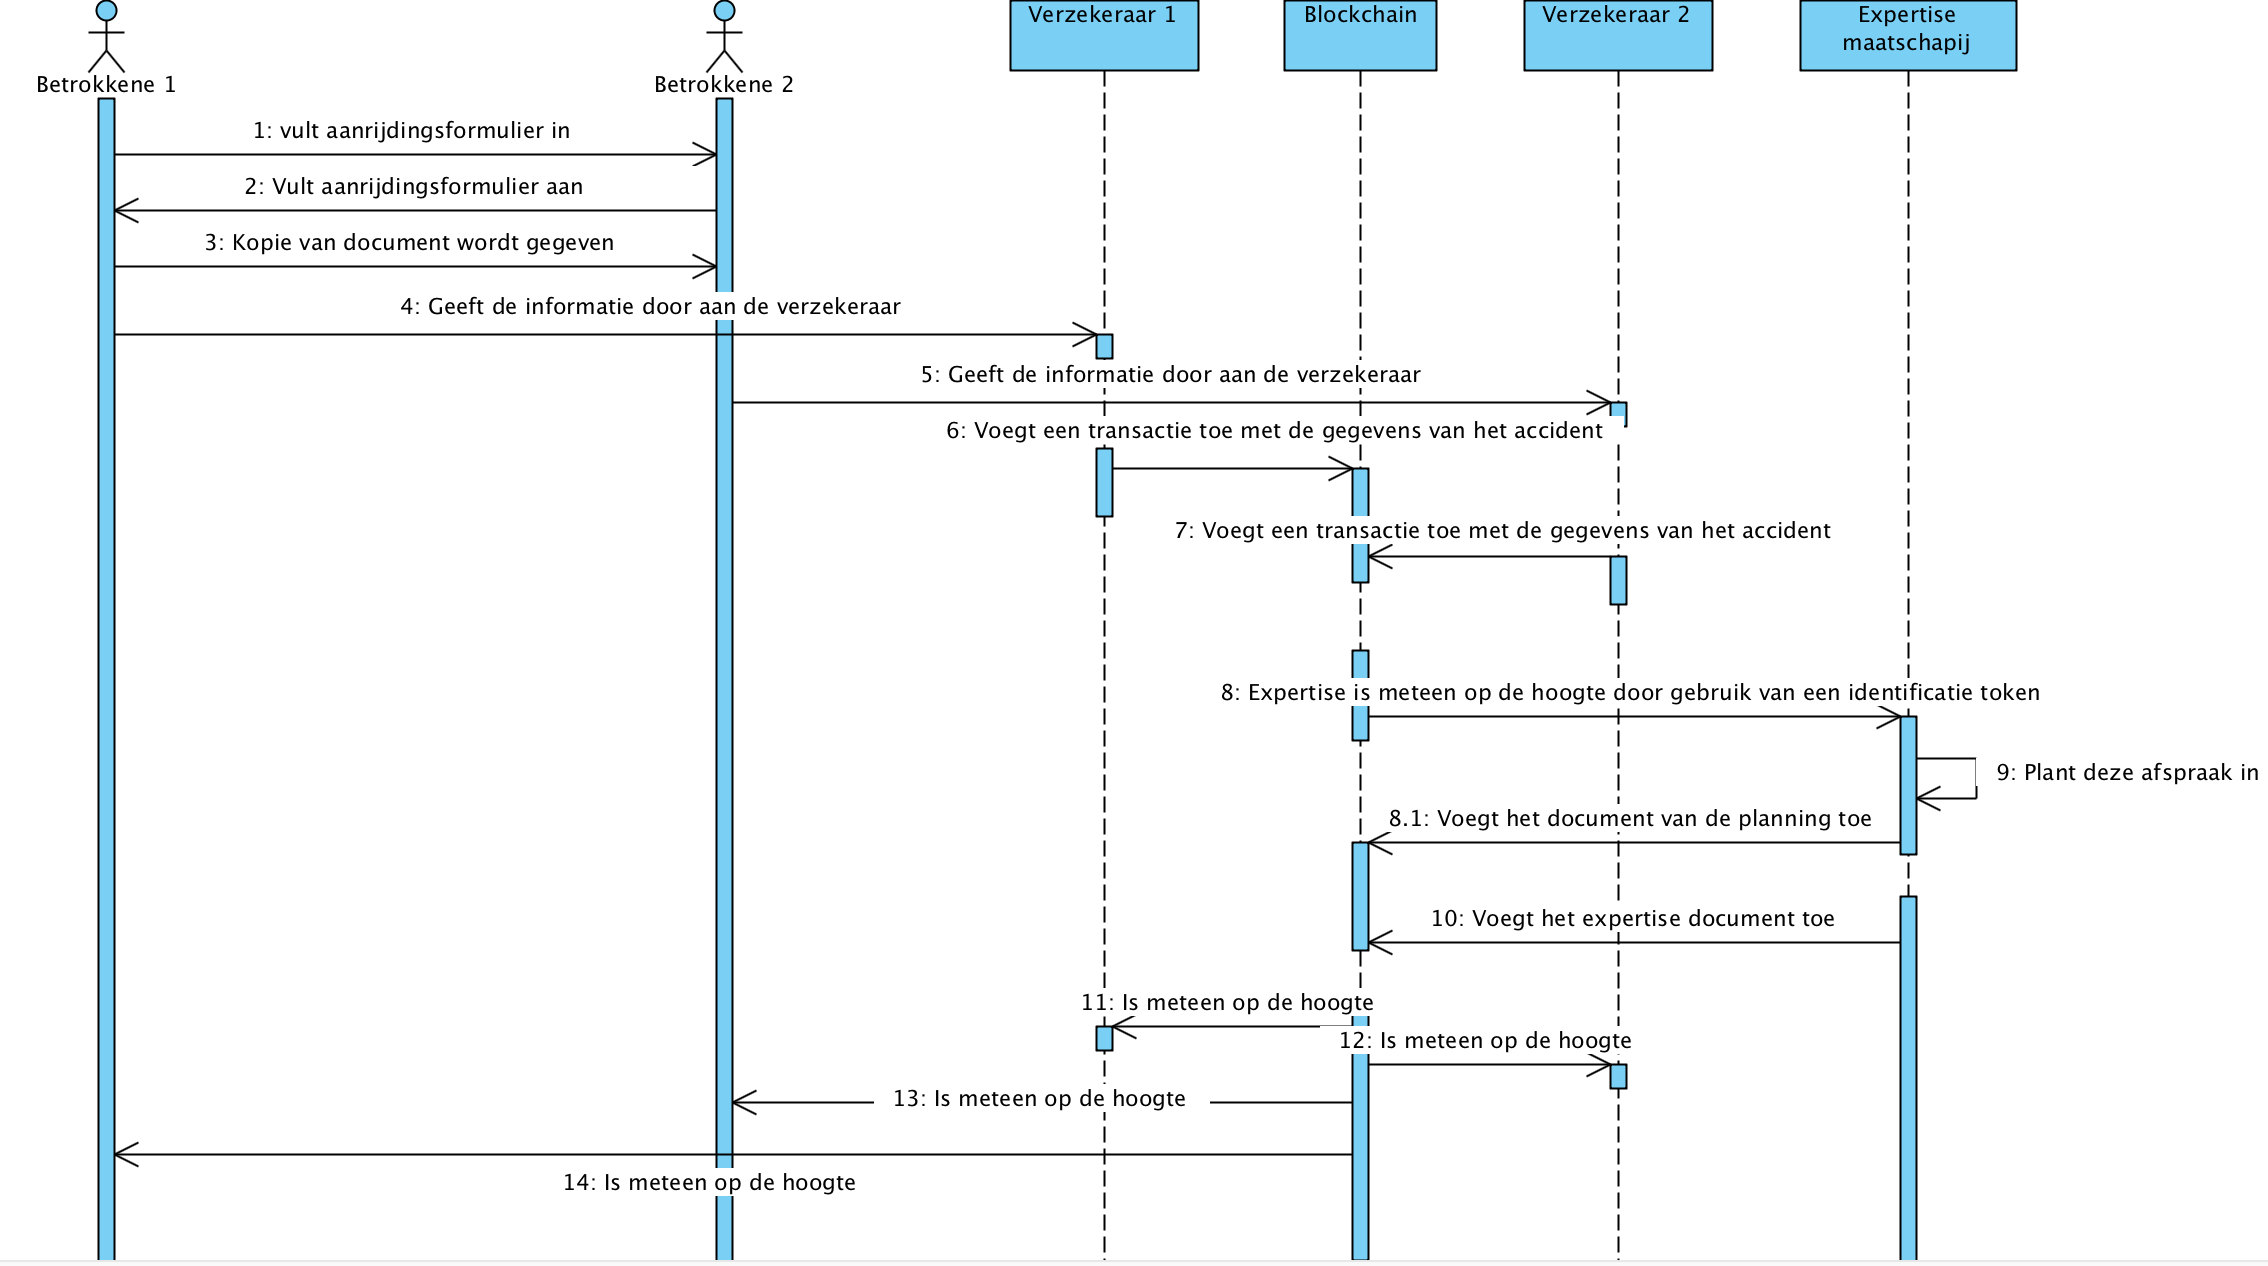
\includegraphics[width=\linewidth]{sd-ongeluk-blockchain.png}
	\caption{Een sequentie diagram dat aantoont hoe de communicatie verloopt bij het aangeven van een auto ongeluk wanneer men gebruik maakt van blockchain.}
	\label{fig:accident-blockchain}
\end{figure}

Door meteen ook de betrokkene personen toegang te geven tot een platform kunnen deze het volledige proces volgen en wordt men sneller op de hoogte gehouden. Ook zal het oplossen van dossiers sneller opgelost worden op deze manier. Een alternatief verloop is te zien op Figuur \ref{fig:accident-blockchain}.

\subsection{Veranderen van verzekering}
Door op deze manier blockchain te gaan gebruiken zijn er nog meer voordelen. Stel dat je van verzekering wil veranderen dan moet deze verzekering eerst een attest bezorgen over het rijgedrag van die cliënt indien deze meteen dezelfde bonus wil aanhouden als bij zijn huidige verzekering. Ook dit kan opgelost worden met blockchain aangezien alle aanrijdingen ook zijn opgenomen in de blockchain en de andere verzekeringspartij deze dus rechtstreeks kan opvragen. 

\section{Aankoop van een nieuwe wagen}
Wanneer men een auto aankoopt en deze wil laten in verkeer stellen en verzekeren is er een heleboel papierwerk nodig. Zo moet er een nummerplaat worden aangevraagd indien deze nog niet ter beschikking is, je moet je wagen zelf laten verzekeren, je wagen moet aangegeven worden om deze in het verkeer te stellen. Dit zijn meteen een heleboel documenten die samen één doel hebben. Het toelaten voor met een wagen op de openbare weg te rijden. Dit kan natuurlijk allemaal makkelijker gemaakt worden door gebruik van blockchain. 

Zo worden de papieren verzekeringspapieren bijvoorbeeld overbodig alsook documenten van in verkeerstelling. Men kan een wagen laten verzekeren bij een verzekeraar, vervolgens kan deze de aanvraag toevoegen aan de blockchain. Alle andere partijen zien hierdoor ook meteen op de hoogte van de aanvraag en kunnen deze meteen verwerken. Het is hierdoor dus ook meteen niet langer nodig om een papieren verzekeringsbewijs of inschrijvingsbewijs bij te houden in de wagen of te wachten tot je de juiste papieren ontvangen hebt.

Bij een politiecontrole is het bijvoorbeeld ook mogelijk om de gegevens op te halen via een applicatie en te kijken of alle documenten in orde zijn van de wagen aangezien alle documenten meteen gegroepeerd zijn. 

\chapter{Alternatieve Technologieën}
\label{ch:alternative-technology}

\section{Hashgraph}
Hashgraph is een technologië met net dezelfde visie als blockchain. Het decentraliseert data om de communicatie tussen verschillende partijen te vergemakkelijken. 

Hashgraph wordt ook aanzien als een verbetering op de problemen die zich voordoen bij blockchain. Zo is blockchain niet heel snel in het verwerken van transacties op een publiek netwerk door het gebruik van proof of work. Verder weet elke node ook niet van elkaar of de transactie geslaagd is aangezien deze transactie verwerkt wordt door een andere node. 

Hashgraph biedt hier een oplossing voor door gebruik te maken van een ``gossip protocol''.

\subsection{Gossip protocol}
Het gossip protocol zorgt ervoor dat elke node op de hoogte gehouden wordt van een verandering op het netwerk. Wanneer één node een verandering waarneemt zal deze willekeurig een andere node selecteren en deze informatie meedelen aan deze node. De node die de verandering ontving zal op zijn beurt hetzelfde doen en een andere node willekeurig selecteren en deze alles wat hij weet mededelen. De node die de verandering oorspronkelijk als eerste verstuurde zal dit repetitief blijven doen net zoals elke andere ingelichte node. Op deze manier zal de verandering exponentieel verspreiden over het netwerk.

Om de werking van het gossip protocol duidelijk te maken wordt er een voorbeeld opstelling gebruikt. In het netwerk bevinden zich 5 nodes respectievelijk An, John, Wim, Karel, Alice.
An ondervindt als eerste node een verandering, An kiest vervolgens willekeurig een andere node, in dit geval Karel. An vertelt Karel alles wat zij weet. Vervolgens doet Karel net hetzelfde, hij kiest willekeurig een node en vertelt deze alles wat hij weet. Ondertussen doet An dit ook, ze kiest een andere willekeurige node en vertelt deze ook alles. Op Figuur \ref{fig:hashgraph-gossip} is deze opstelling visueel te zien.

\begin{figure}
	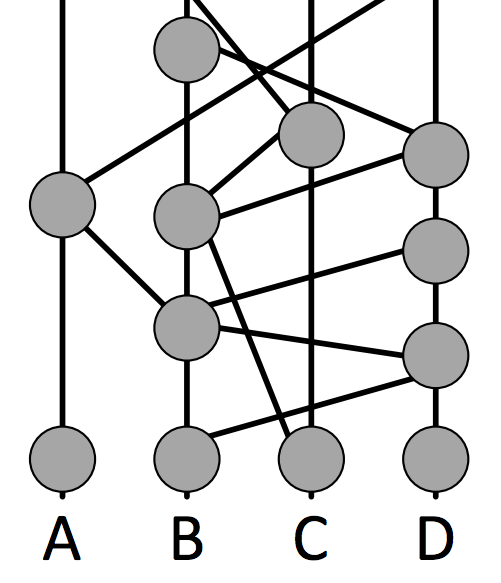
\includegraphics[width=\linewidth]{hashgraph-communication.png}
	\caption{Een visuele weergave van het gossip protocol \textcite{Baird2016}.}
	\label{fig:hashgraph-gossip}
\end{figure}

De hashgraph is meteen ook de data structuur die alle gossip bijhoudt, zo weet elke node ook welke gossip gebeurt is tussen verschillende nodes. Op deze manier worden er ook geen gossip uitgevoerd naar nodes die al op de hoogte zijn van de verandering. Verder weet ook elke node wanneer welke node met een andere node gossip uitvoerde, op deze manier kunnen andere transacties die ondertussen al gebeurd zijn ook toegevoegd worden op de juiste plaats.
Als dit principe nog verder bekeken wordt dan weet een node dus ook of de geselecteerde node de voorgaande transacties ook al weet of niet \textcite{Baird2016a}.

\subsection{Overeenkomst algoritme}
Bij een hashgraph is het niet nodig om een bepaalde ``stem'' over het netwerk te sturen. Elke node heeft een kopie van dezelfde  hashgraph. Wanneer 2 nodes dezelfde hashgraph hebben 
wordt er ook meteen een akkoord behaald. 

Natuurlijk kan het altijd zijn dat één node al transacties heeft opgenomen in de hashgraph die de andere nog niet heeft opgenomen. Dit probleem wordt opgelost door gebruik te maken van ``virtual voting'' \textcite{Baird2016a}.

\subsection{Virtual voting}
Stel dat node A een versie heeft van de hashgraph en node B een gelijkaardige versie heeft van de hashgraph. Beide kunnen verschillen maar zullen over het algemeen consistent zijn. Hiermee wordt bedoeld dat wanneer beide hashgraphs een transactie hebben dat de``ouder'' van deze transactie dezelfde is en dat bovendien de ouder van deze transactie ook dezelfde zal zijn en dit voor alle overeenkomende transacties. 

Als beide nodes vertrouwbare nodes zijn dan wordt er vanuit gegaan dat de ene node deze transactie ook snel te weten zal komen. Het hele systeem werkt asynchroon dus er wordt geen rekening gehouden met hoe snel dit gebeurt.

Wanneer dus beide hashgraphs niet gelijk zijn aan elkaar wordt er virtual voting toegepast. Hier zal de node enkele verkiezingen opstellen met evenementen. Om deze werking te verklaren worden eerst enkele principes uitgelegd \textcite{Baird2016a}.

\subsubsection{Rounds}
Hashgraph maakt gebruik van rounds. Een round of ronde wordt bij elk evenement gegenereerd. Een kind van een evenement zal ook nooit een lager nummer hebben dan dat van de ouder aangezien dit steeds na de ouder aangemaakt zal zijn. Bij elk evenement dat wordt aangemaakt zal dus de ronde stijgen of hetzelfde blijven maar zal dit nooit dalen
\textcite{Baird2016}. Op Figuur \ref{fig:hashgraph-rounds} is een voorbeeld te zien van rounds.

\begin{figure}
	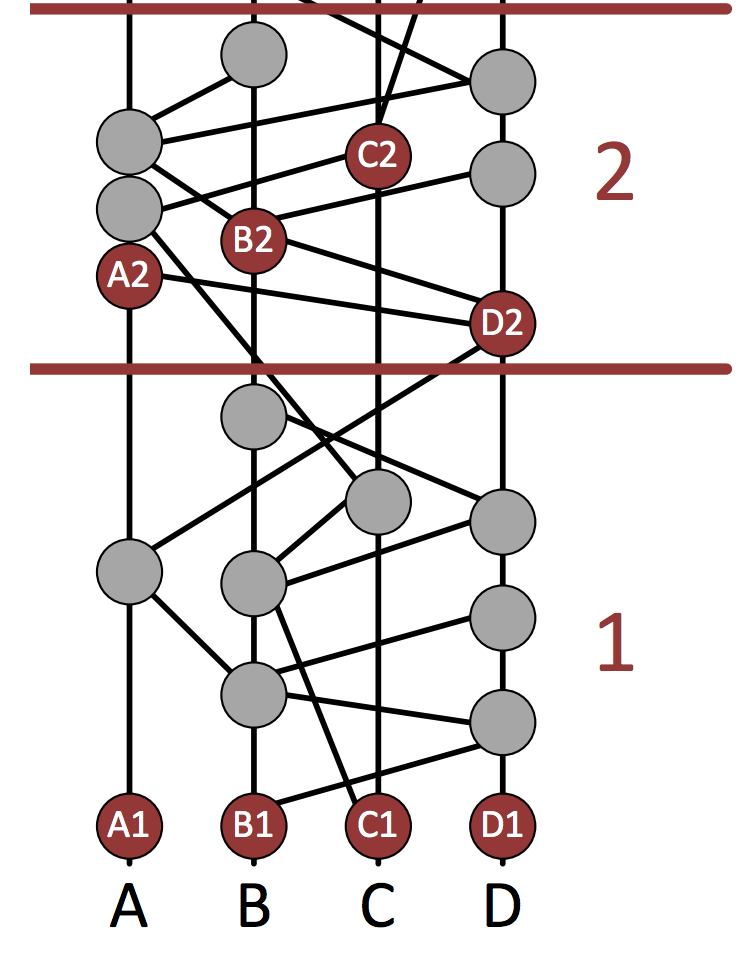
\includegraphics[width=\linewidth]{hashgraph-rounds.png}
	\caption{Een visuele weergave van rounds \textcite{Baird2016}.}
	\label{fig:hashgraph-rounds}
\end{figure}

\subsubsection{Witness}
Verder wordt er ook gebruik gemaakt van een ``witness'' of een getuige. Het eerste evenement dat wordt aangemaakt in een ronde noemt men een getuige. Alle andere nodes genereren deze ook voor zichzelf. Verder moet er ook voor elke getuige berekend worden of deze getuige ook een beroemde getuige is. 
\textcite{Baird2016}

\subsubsection{Famous witness}
Stel er zijn 4 nodes respectievelijk A, B, C, D. Zoals eerder vermeld worden er ook telkens rondes berekend en is elk eerste evenement van elke node een getuige. Wanneer er wilt gekeken worden of B2 een beroemde getuige is wordt het volgende gedaan. Er wordt gekeken naar de getuigen van de volgende ronde (in dit geval ronde 3). De getuige wordt dan als beroemd gezien als deze veel voorkomt bij de getuigen van de volgende ronde. Op deze manier wordt dit berekend voor elke getuige om zijn beroemdheid te meten
\textcite{Baird2016}. Een visuele weergave is te zien op Figuur \ref{fig:hashgraph-famouswitness}.

\begin{figure}
	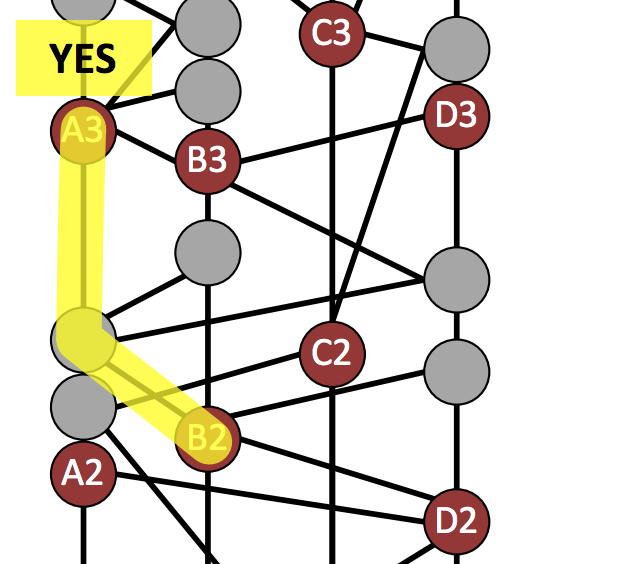
\includegraphics[width=\linewidth]{hashgraph-famouswitness.png}
	\caption{Een visuele weergave van een famous witness \textcite{Baird2016}.}
	\label{fig:hashgraph-famouswitness}
\end{figure}


\subsubsection{Bedriegen van het syteem}
Er is uiteraard een andere manier waar nodes mee kunnen bedriegen. Stel dat een node een bepaald evenement aanmaakt maar hier de vorige hash gebruikt van een vorig evenement dat hij zelf aanmaakte in plaats van de ouder in te stellen als het evenement zelf. Op deze manier verbreekt hij de ketting en maakt hij een boom structuur. 

Wanneer deze node vervolgens bedriegt bij het gossip protocol en hier verkeerde informatie doorgeeft dan zullen er later bij het virtual voting systeem ook fouten opduiken aangezien de andere nodes verschillen zullen hebben. Op deze manier zullen deze nodes dus ook niet meer tot een overeenkomst komen voor een tijdje \textcite{Baird2016a}.

\subsection{Eerlijkheid in het systeem}
Hashgraph is ook een eerlijk systeem, dit wil zeggen dat het eerlijk de nodes zal kiezen. 
Waar bij blockchain gebruik gemaakt werd van wie het eerst de proof-of-work genereerde wordt hier een verschil gemaakt. 

Bij hashgraph gaat het niet om wie het eerst de transactie aanmaakt maar eerder hoeveel andere nodes deze bereikt heeft. Stel dat er een transactie wordt verzonden en deze wordt opgelost door een systeem dat de verbinding met internet verbreekt en dus deze transactie niet kan verzenden en voor zich houdt dan treden er problemen op aangezien bij proof of work deze node eerst zou zijn. Een andere node wordt uiteraard gekozen die het eerst deze transactie terug broadcast. Wanneer later deze node die de verbinding verbrak terug online komt en deze transactie broadcast dan zal dit overal moeten aangepast worden aangezien eigenlijk deze node eerst een ``timestamp'' genereerde die eerder valt dan de oorspronkelijk gekozen tijdstempel. 

Door gebruik te maken van wiens transactie het meeste nodes bereikt van het totale netwerk en vervolgens ook deze te kiezen bekomt men een eerlijk systeem. De eerste die deze transactie verstuurt zal in het algemeen ook als eerste een grootste deel van het netwerk kunnen bereiken door gossip \textcite{Baird2016a}.

\subsection{Verschillen met blockchain?}
De verschillen met blockchain zijn vooral de snelle communicatie en het stemmen over de juistheid van de transacties. Verder worden er ook geen ``blocks'' gebruikt bij hashgraph maar wordt dit een ``evenement'' genoemd \textcite{Baird2016a}.

Verder is het hele systeem ook volledig anders opgebouwd en zijn beide in theorie niet te vergelijken. Het doel van beide is hetzelfde, het decentraliseren van data. 